%============================================================================
% MacBook Pro 16" Thermal/Airflow CFD — IEEEtran conference-style write-up.
%
% Compilation:
%   # Recommended — XeLaTeX or LuaLaTeX
%   # (Charter body + STIX Two Math + JetBrains Mono code)
%   xelatex  macbook_cfd_report.tex
%   xelatex  macbook_cfd_report.tex         (second pass for cross-refs)
%
%   # Fallback — pdflatex
%   # (Charter via mathdesign + Inconsolata as monospace substitute)
%   pdflatex macbook_cfd_report.tex
%   pdflatex macbook_cfd_report.tex
%
% All three font families are embedded in the output PDF automatically.
%============================================================================

\documentclass[10pt,twocolumn,letterpaper]{article}

% ---------------------------------------------------------------------------
% Page geometry — margins, column separation, header/footer space.
% ---------------------------------------------------------------------------
\usepackage[margin=0.85in,top=0.65in,bottom=0.85in,headheight=14pt,%
            headsep=8pt,columnsep=0.28in]{geometry}

% ---------------------------------------------------------------------------
% Font stack. XeLaTeX/LuaLaTeX path uses the full OpenType fonts; pdflatex
% path uses Bitstream Charter via the mathdesign package.
% ---------------------------------------------------------------------------
\usepackage{iftex}
\ifPDFTeX
  \usepackage[T1]{fontenc}
  \usepackage[utf8]{inputenc}
  \usepackage[bitstream-charter]{mathdesign}   % Charter body + math
  \usepackage{inconsolata}                      % monospace fallback
\else
  \usepackage{fontspec}
  \usepackage{unicode-math}
  \setmainfont{Charter}
  \setmathfont{STIX Two Math}
  % Prefer JetBrains Mono; fall back to Menlo if it isn't installed.
  \IfFontExistsTF{JetBrains Mono}
    {\setmonofont{JetBrains Mono}[Scale=0.88]}
    {\setmonofont{Menlo}[Scale=0.85]}
\fi
\usepackage{microtype}

% ---------------------------------------------------------------------------
% Line spacing and heading-orphan guards (addresses rendering bugs):
%   - \linespread{1.08}    slight line-spacing bump so sub/superscripts
%                          do not crowd adjacent baselines.
%   - needspace            lets every heading declare a minimum amount of
%                          content that must follow in the same column.
%   - nowidow              catches widow/orphan lines as a second net.
%   - \emergencystretch    lets the justifier relax spacing before
%                          breaking words badly, eliminating rivers of
%                          whitespace in narrow columns.
% ---------------------------------------------------------------------------
\linespread{1.08}
\usepackage{needspace}
\usepackage{balance}
\usepackage[defaultlines=3,all]{nowidow}
\setlength{\emergencystretch}{3em}
\hyphenpenalty=50
\tolerance=1500
\raggedbottom

% ---------------------------------------------------------------------------
% Math
% ---------------------------------------------------------------------------
\usepackage{amsmath}
\ifPDFTeX
  \usepackage{amssymb}
\fi
\usepackage{bm}
% Display math uses the 10pt body-text size so equations do not look
% pinched. Ensure no amsmath environment forces smaller script sizes.
\DeclareMathSizes{10}{10}{7.5}{6}

% ---------------------------------------------------------------------------
% Units
% ---------------------------------------------------------------------------
\usepackage{siunitx}
\DeclareSIUnit{\inch}{in}
\sisetup{
  per-mode       = symbol,
  detect-all,
  range-phrase   = \text{\textendash},
  range-units    = single,
}

% ---------------------------------------------------------------------------
% Tables and figures
% ---------------------------------------------------------------------------
\usepackage{booktabs}
\usepackage{array}
\usepackage{tabularx}
\usepackage{graphicx}
\graphicspath{{../figures/}{./figures/}{./}}
\usepackage{float}
\usepackage[labelfont=bf,font=small]{caption}
\usepackage{subcaption}
\usepackage{threeparttable}
\usepackage[hidelinks]{hyperref}
\usepackage{xcolor}
\usepackage{mdframed}

% Force long form caption labels to match "Figure" convention.
\renewcommand{\tablename}{Table}
\renewcommand{\figurename}{Figure}
\captionsetup[table]{name=Table,labelsep=colon}
\captionsetup[figure]{name=Figure,labelsep=colon}

% ---------------------------------------------------------------------------
% Running header + footer page number (spring-report style).
% ---------------------------------------------------------------------------
\usepackage{fancyhdr}
\pagestyle{fancy}
\fancyhf{}
\fancyhead[L]{\small\itshape Two- and Three-Dimensional Chassis CFD}
\fancyhead[R]{\small\itshape MacBook Pro 16-inch under Sustained Load}
\renewcommand{\headrulewidth}{0.4pt}
\fancyfoot[C]{\small\thepage}
\fancypagestyle{plain}{%
  \fancyhf{}%
  \fancyhead[L]{\small\itshape Two- and Three-Dimensional Chassis CFD}%
  \fancyhead[R]{\small\itshape MacBook Pro 16-inch under Sustained Load}%
  \renewcommand{\headrulewidth}{0.4pt}%
  \fancyfoot[C]{\small\thepage}%
}

% ---------------------------------------------------------------------------
% Arabic section numbering with trailing period (spring-report style).
% "1. Introduction", "2.1. Design Variables", etc.
% ---------------------------------------------------------------------------
\usepackage{titlesec}
\titleformat{\section}[hang]
  {\normalfont\large\bfseries}{\thesection.}{0.6em}{}
\titleformat{\subsection}[hang]
  {\normalfont\normalsize\bfseries}{\thesubsection.}{0.5em}{}
\titlespacing*{\section}{0pt}{0.7em}{0.25em}
\titlespacing*{\subsection}{0pt}{0.5em}{0.2em}

% ---------------------------------------------------------------------------
% Abstract as "\textbf{Abstract.}" run-in paragraph spanning full page,
% wrapped in a subtle grey mdframed box.
% ---------------------------------------------------------------------------
\definecolor{abstractbg}{gray}{0.93}
\newmdenv[
  backgroundcolor=abstractbg,
  linewidth=0pt,
  leftmargin=0pt,
  rightmargin=0pt,
  innerleftmargin=10pt,
  innerrightmargin=10pt,
  innertopmargin=8pt,
  innerbottommargin=8pt,
  skipabove=0pt,
  skipbelow=4pt,
]{abstractbox}
\renewenvironment{abstract}%
  {\begin{abstractbox}\noindent\textbf{Abstract.}\hspace{0.6em}\ignorespaces}%
  {\end{abstractbox}}

% ---------------------------------------------------------------------------
% Spacing
% ---------------------------------------------------------------------------
\setlength{\parskip}{3pt}
\setlength{\parindent}{0pt}
\setlength{\textfloatsep}{4pt plus 1pt minus 1pt}
\setlength{\floatsep}{3pt plus 1pt minus 1pt}
\setlength{\intextsep}{3pt plus 1pt minus 1pt}
\setlength{\dblfloatsep}{3pt plus 1pt minus 1pt}
\setlength{\dbltextfloatsep}{4pt plus 1pt minus 1pt}
\setlength{\abovecaptionskip}{4pt}
\setlength{\belowcaptionskip}{0pt}

% Loosen float-placement limits so large figure* blocks aren't all
% deferred to the end.
\setcounter{topnumber}{4}
\setcounter{bottomnumber}{3}
\setcounter{totalnumber}{6}
\setcounter{dbltopnumber}{4}
\renewcommand{\topfraction}{0.95}
\renewcommand{\bottomfraction}{0.85}
\renewcommand{\textfraction}{0.08}
\renewcommand{\floatpagefraction}{0.75}
\renewcommand{\dbltopfraction}{0.95}
\renewcommand{\dblfloatpagefraction}{0.75}

% ---------------------------------------------------------------------------
% Shortcuts
% ---------------------------------------------------------------------------
\newcommand{\ubf}{\mathbf{u}}
\newcommand{\fB}{\mathbf{f}_{B}}
\newcommand{\uT}{\mathbf{u}_{\mathrm{target}}}
\newcommand{\Sbm}{\mathbf{S}}
\newcommand{\nueff}{\nu_{\mathrm{eff}}}
\newcommand{\nut}{\nu_{t}}
\newcommand{\qsrc}{\dot{q}^{\prime\prime\prime}}
\newcommand{\Ra}{\mathrm{Ra}}
\newcommand{\Reyn}{\mathrm{Re}}
\newcommand{\Gr}{\mathrm{Gr}}
\newcommand{\Pran}{\mathrm{Pr}}
\newcommand{\Linf}{L_{\infty}}
\newcommand{\kchas}{k_{\mathrm{chassis,\,active}}}
\newcommand{\kTIM}{k_{\mathrm{TIM}}}
\newcommand{\vfan}{v_{\mathrm{fan}}}

% ===========================================================================
\begin{document}
% ===========================================================================

% Custom title block (spring-report style): centred title over a
% single-line "Name | Institution" author row, no date.
\makeatletter
\renewcommand{\@maketitle}{%
  \begin{center}
    {\LARGE\bfseries\@title\par}
    \vspace{0.6em}
    {\normalsize \@author\par}
  \end{center}%
  \vspace{0.2em}%
}
\makeatother

\title{Two- and Three-Dimensional CFD of a MacBook Pro 16-inch
       Chassis under Sustained CPU Load}
\author{Jaehyeok Kim \quad\textbar\quad Georgia Institute of Technology}
\date{}

\makeatletter
\twocolumn[%
  \begin{@twocolumnfalse}
  \@maketitle
  \begin{abstract}
  Two finite-volume CFD solvers (2D and 3D) are developed to predict
  the thermal field of a MacBook Pro 16-inch under sustained CPU load.
  The 2D top-down formulation uses a 1D out-of-plane closure; the 3D
  formulation resolves the vertical dimension directly. Both use
  staggered MAC grids, pseudo-transient Chorin projection with implicit
  Brinkman penalization, and direct sparse LU factorization of the
  pressure-correction Poisson equation. A three-level grid refinement
  study confirms that the lateral thermal metrics are mesh-converged
  (GCI\,$\le$\,\SI{1.7}{\percent}). Predictions for the four thermal
  metrics---SoC die, battery maximum, palm-rest surface, and exhaust
  air---agree with published ranges compiled from up to five
  independent sources (per-metric counts in Table~\ref{tab:valid})
  to within \SI{1.2}{\celsius}.
  The 2D model predicts SoC\,$=\SI{96}{\celsius}$; the 3D model
  predicts \SI{81}{\celsius}; the published range is
  82--98\,\si{\celsius}. The 2D/3D spread reflects the additional
  surface area resolved in 3D.
  \end{abstract}
  \vspace{8pt}
  \end{@twocolumnfalse}
]
\makeatother

% ===========================================================================
\needspace{2\baselineskip}
\section*{Nomenclature}
% ===========================================================================

\renewcommand{\arraystretch}{1.15}
\noindent
\begin{tabularx}{\columnwidth}{@{}l@{\hspace{8pt}}X@{}}
$\ubf$                         & Velocity vector, \si{m/s} \\
$u, v, w$                      & Velocity components in $x,y,z$, \si{m/s} \\
$\uT$                          & Target velocity in pinned faces, \si{m/s} \\
$p,\;\delta p$                 & Pressure / pressure correction, \si{Pa} \\
$T$                            & Temperature, \si{\celsius} or \si{K} \\
$\rho$                         & Density, \si{kg\per\cubic\meter} \\
$\mu$                          & Dynamic viscosity, \si{Pa.s} \\
$\nu$                          & Kinematic viscosity, \si{\square\meter\per\second} \\
$\nut$                         & Eddy viscosity (mixing length), \si{\square\meter\per\second} \\
$\nueff$                       & Effective viscosity $\nu+\nut$, \si{\square\meter\per\second} \\
$\ell_{m}$                     & Mixing length, \si{m} \\
$\beta$                        & Brinkman penalty coefficient, \si{\per\second} \\
$k$                            & Thermal conductivity, \si{W\per\meter\per\kelvin} \\
$c_{p}$                        & Specific heat, \si{J\per\kilogram\per\kelvin} \\
$\alpha$                       & Thermal diffusivity $k/(\rho c_{p})$, \si{\square\meter\per\second} \\
$\qsrc$                        & Volumetric heat source, \si{\watt\per\cubic\meter} \\
$h$                            & Grid spacing, \si{m} \\
$\Delta t$                     & Pseudo-time step, \si{s} \\
$\alpha_{u},\;\alpha_{p}$      & Momentum / pressure relaxation (2D: 0.7/0.8; 3D: 0.6/0.8) \\
$\Reyn$                        & Reynolds number, $\rho U L/\mu$ \\
$\Pran$                        & Prandtl number, $\nu/\alpha$ \\
$\Ra$                          & Rayleigh number, $g\beta_{T}\,\Delta T\,L^{3}/(\nu\alpha)$ \\
$\Gr$                          & Grashof number, $\Ra/\Pran$ \\
$\mathrm{GCI}$                 & Grid convergence index \cite{roache1994}, \si{\percent} \\
\end{tabularx}

% ===========================================================================
\section{Introduction}
% ===========================================================================

Thin-and-light laptops dissipate
\SIrange{15}{60}{\watt} of heat from chips that occupy less than
\SI{100}{\square\milli\meter} of die area. Maintaining junction
temperatures below the \SI{100}{\celsius} throttle threshold requires
careful co-design of heat pipes, vapor chambers, fan blowers, and
chassis aluminum. Accurate thermal modelling enables engineers to
evaluate heat-spreader geometry, thermal-interface materials, and
cooling strategies before physical prototyping.

This work develops two finite-volume CFD models of a
\SI{16}{\inch} MacBook Pro chassis and compares the predicted
thermal field to published thermal-imaging data. The 2D model
approximates the out-of-plane dimension with a 1D closure:
volumetric heat sources are scaled by an effective slab thickness
and lateral conduction uses an effective chassis conductivity. The
3D model resolves the thickness explicitly on a
$90 \times 62 \times 16$ grid, using bounding-box components for
the battery stack, logic board, vapor chamber, and fin-stack
radiator. The shared top-down component layout used by both models
is shown in Figure~\ref{fig:layout}.

Both models share the same solver architecture. The 2D/3D comparison
therefore isolates the effect of geometric dimensionality on the
predicted temperature field. This comparison is the paper's primary
contribution and is addressed in Section~\ref{sec:synthesis}.

% ===========================================================================
\needspace{2\baselineskip}
\section{Governing Equations}
\label{sec:gov}
% ===========================================================================

The fluid is modelled as incompressible air with constant
properties. The Rayleigh number based on
$\Delta T = \SI{70}{K}$ and
$L = \SI{10}{mm}$ evaluates to $\Ra \approx \num{5.2e3}$, giving
$\Gr/\Reyn^{2} \approx \num{1.3e-5}$. Because this ratio is much
less than unity, forced convection dominates and buoyancy is
neglected. The governing equations are continuity, incompressible
momentum, and steady-state energy:
%
\begin{equation}
  \nabla\cdot\ubf = 0.
  \label{eq:continuity}
\end{equation}
%
\begin{equation}
  \frac{\partial \ubf}{\partial t}
  + (\ubf\cdot\nabla)\ubf
  = -\frac{1}{\rho}\nabla p
    + \nabla\!\cdot\!(\nueff\,\nabla\ubf)
    + \fB.
  \label{eq:momentum}
\end{equation}
%
\begin{equation}
  \rho\,c_{p}\,\ubf\cdot\nabla T
  = \nabla\!\cdot\!(k\,\nabla T) + \qsrc.
  \label{eq:energy}
\end{equation}
%
The Brinkman penalization~\cite{angot1999} pins face velocities
inside solid bodies, fan cells, and the inlet patch:
%
\begin{equation}
  \fB = -\beta\,(\ubf - \uT),
  \label{eq:brinkman}
\end{equation}
%
with $\beta = \SI{e5}{\per\second}$ where pinned and zero elsewhere.

% ===========================================================================
\needspace{2\baselineskip}
\section{Numerical Method}
\label{sec:num}
% ===========================================================================

\needspace{2\baselineskip}
\subsection{Staggered MAC grid}

On the staggered MAC grid of Harlow and Welch~\cite{harlow1965},
pressure and temperature are stored at cell centres; velocity
components are stored at cell faces. The staggered arrangement
eliminates odd--even decoupling in the pressure--velocity coupling.

\needspace{2\baselineskip}
\subsection{Turbulence closure}

The algebraic mixing-length model is used in 2D:
%
\begin{equation}
  \nut = \ell_{m}^{2}\,|\Sbm|,
  \qquad
  |\Sbm| = \sqrt{2\,\Sbm\!:\!\Sbm},
  \label{eq:mixing}
\end{equation}
%
where $\Sbm$ is the symmetric strain-rate tensor and
$\ell_{m} = \SI{4}{mm}$ is the mixing length
($\approx$\,1.6\,\si{\percent} of domain height). The eddy viscosity
is capped at $\nut/\nu \le 80$ to prevent unphysical blow-up in
highly sheared cells. Turbulence is disabled in the 3D model
($\nut = 0$) because the coarser grid cannot resolve shear-layer
structure at this length scale. This simplification is acceptable
at $\Reyn \approx \num{24e3}$ for bulk temperature predictions.

\needspace{2\baselineskip}
\subsection{Pseudo-transient Chorin projection}
\label{sec:chorin}

The pressure--velocity coupling follows the fractional-step
(projection) method of Chorin~\cite{chorin1968}. Each pseudo-time
step applies four substeps. First, a momentum predictor with
explicit first-order upwind advection, conservative
variable-viscosity diffusion, previous-step pressure gradient, and
implicit Brinkman drag:
%
\begin{equation}
  \ubf^{\,*} \;=\; \dfrac{\ubf^{n}
                   \,+\, \Delta t\,\mathbf{R}(\ubf^{n},p^{n})
                   \,+\, \Delta t\,\beta\,\uT}
                  {1 \,+\, \Delta t\,\beta}.
  \label{eq:predictor}
\end{equation}
%
Second, a SIMPLE-style under-relaxation~\cite{patankar1980} of the
predictor before projection, with momentum relaxation
$\alpha_{u}=0.7$ (2D) or $0.6$ (3D):
%
\begin{equation}
  \ubf^{\,*} \leftarrow \ubf^{n} + \alpha_{u}\,(\ubf^{\,*}-\ubf^{n}).
  \label{eq:urelax}
\end{equation}
%
Third, a pressure-correction Poisson solve on flow cells:
%
\begin{equation}
  \nabla^{2}\,\delta p
  = \frac{\rho}{\Delta t}\,\nabla\!\cdot\!\ubf^{\,*},
  \label{eq:poisson}
\end{equation}
%
with Neumann conditions at walls, solids, and the inlet (drop the
face coefficient) and Dirichlet $\delta p = 0$ at outlet faces.
Disconnected fluid pockets without a Dirichlet anchor are pinned
by row--identity substitution. Fourth, a velocity correction
$\ubf^{n+1} = \ubf^{\,*} - (\Delta t/\rho)\,\nabla\delta p$,
followed by a hard re-pin of Brinkman faces. Pressure is updated
with $p^{n+1} = p^{n} + \alpha_{p}\,\delta p$, $\alpha_{p} = 0.8$.

The pseudo-time step satisfies a combined convective/viscous CFL
constraint:
%
\begin{equation}
  \Delta t = \min\!\left(
    \mathrm{CFL}\,\frac{h}{|\ubf|_{\max}},\;
    \frac{1}{4}\,\frac{h^{2}}{\nueff^{\max}}\right),
  \label{eq:cfl}
\end{equation}
%
with $\mathrm{CFL} = 0.35$ (2D) or $0.30$ (3D).

\needspace{2\baselineskip}
\subsection{Pressure Poisson solver}

The Poisson matrix is assembled once from the 5-point (2D) or
7-point (3D) stencil on cells inside the flow mask. Both dimensions
use direct LU factorization via SciPy's \texttt{splu}~\cite{scipy};
the factorization is reused for every pseudo-time step because the
matrix is static. At $n \approx \num{19e3}$ (2D) and
$n \approx \num{63e3}$ (3D) flow-cell unknowns, the fill-in remains
manageable on a laptop ($<$\,\SI{100}{MB}). This design eliminates
the convergence fragility of iterative CG/Jacobi solvers.

\needspace{2\baselineskip}
\subsection{Energy equation}

Temperature is computed via a steady-state solve once the velocity
field has converged. First-order upwind is used for advection
(Peclet-robust, diagonally dominant); harmonic-mean face
conductivity is used for diffusion. The harmonic mean represents
sharp conductivity jumps between high-$k$ metal
($k = \SI{2000}{W\per\meter\per\kelvin}$, vapor chamber) and low-$k$ air
($k = \SI{0.028}{W\per\meter\per\kelvin}$) without Gibbs-style
artefacts at component boundaries.

\needspace{2\baselineskip}
\subsection{Convergence diagnostics}

Two independent residuals are tracked. The first is the
$\Linf$ divergence on \emph{deep interior} flow cells---cells whose
four (2D) or six (3D) face neighbours are all inside the flow mask---which measures
true mass conservation. The second is the $\Linf$ momentum update
$\max\lvert\ubf^{n+1}-\ubf^{n}\rvert$, which measures approach to
steady state. A run is declared converged when both fall below
prescribed tolerances. The separate treatment avoids conflating
Brinkman-interface error with solution evolution.

% ===========================================================================
\needspace{2\baselineskip}
\section{Geometry and Boundary Conditions}
\label{sec:geom}
% ===========================================================================

\needspace{2\baselineskip}
\subsection{Domain and grid}

Both models share the same top-down footprint:
$L_{x} = \SI{0.355}{m}$ (lateral, along the keyboard) and
$L_{y} = \SI{0.245}{m}$ (front-to-back, palm-rest to rear hinge).
The 3D model adds $L_{z} = \SI{0.016}{m}$ for chassis depth. Grid
statistics are listed in Table~\ref{tab:grid}.

\begin{table}[!tbp]
  \centering
  \caption{Grid dimensions, runtime, and convergence statistics
           at baseline resolution.}
  \label{tab:grid}
  \small
  \begin{tabular}{@{}lcc@{}}
    \toprule
    Parameter                     & 2D                     & 3D \\
    \midrule
    Grid                          & $260\!\times\!180$     & $90\!\times\!62\!\times\!16$ \\
    Total cells                   & \num{46800}            & \num{89280} \\
    Flow cells                    & \num{18875}            & \num{62736} \\
    Runtime (laptop)              & $\sim\!\SI{6}{s}$      & $\sim\!\SI{45}{s}$ \\
    Iterations                    & \num{1997}             & \num{867} \\
    Interior div.\ $\Linf$ (\si{\per\second})
                                  & $\num{3.9e-13}$        & $\num{1.0e-12}$ \\
    \bottomrule
  \end{tabular}
\end{table}

\needspace{2\baselineskip}
\subsection{Components and power}

The 2D model uses twenty-two components to represent the SoC
(\SI{15}{\watt}), dual RAM modules (\SI{2}{\watt} each), dual fan
blowers, vapor chamber
($k = \SI{2000}{W\per\meter\per\kelvin}$), logic board, SSD and
Thunderbolt controllers, speakers, and six battery cells. The 3D
model uses twenty-one components; it omits the Thunderbolt
controllers, power controller, and top vapor-chamber strip, and
adds a central vapor-chamber slab, a homogenized exhaust fin
stack, and a thermal-interface-material (TIM) layer above the
SoC die with
$\kTIM = \SI{0.14}{W\per\meter\per\kelvin}$ in a \SI{1}{mm}-thick
slab, yielding $R_{jc} \approx \SI{9.6}{K\per\watt}$. This
effective resistance is higher than bare-die junction-to-case
values but absorbs unresolved interface resistances in the
die-to-vapor-chamber path.

\needspace{2\baselineskip}
\subsection{Chassis-conductivity closure}

Air cells outside any explicit component inherit an effective bulk
conductivity $k_{\mathrm{chassis}}$ representing unresolved
metallic structure (PCB copper foil, aluminum mounting frame,
thermal pads). The 2D model uses
$\kchas = \SI{3.0}{W\per\meter\per\kelvin}$ and
$k_{\mathrm{chassis,\,battery}} = \SI{0.25}{W\per\meter\per\kelvin}$,
calibrated against published thermal-imaging data. The 3D model
uses a much lower $\kchas = \SI{0.035}{W\per\meter\per\kelvin}$
(near air) because the 3D geometry resolves six heat-loss faces
per component rather than a perimeter.

\needspace{2\baselineskip}
\subsection{Fan boundary condition}
\label{sec:fanbc}

Each fan is modelled as a rectangular volume penalized by
Eq.~\eqref{eq:brinkman}. Both the upstream and downstream $v$-faces
inside the fan region are pinned to the target velocity, producing
a constant axial flow through the fan volume. The target is
$\vfan = \SI{1.2}{m\per\second}$ in 2D and
$\vfan = \SI{2.5}{m\per\second}$ in 3D, calibrated against
published fan-curve data at intermediate RPM. This is an explicit
simplification: a true fan model uses a pressure-rise versus
volumetric-flow curve, whereas the present model prescribes a
fixed flow. The calibrated value is therefore a \emph{tunable
parameter}, not a first-principles input.

\needspace{2\baselineskip}
\subsection{Velocity and thermal boundary conditions}

Velocity BCs: no-slip at all chassis walls; Brinkman-pinned inside
fan cells; Brinkman-pinned inside the inlet patch at
$\SI{1.2}{m\per\second}$ (2D, \SI{195}{mm} line across the
bottom-case vent) or $\SI{1.0}{m\per\second}$ (3D,
$\SI{195}{mm}\!\times\!\SI{4}{mm}$ slit). Outflow at two top-rear
exhaust bands (\SI{88}{mm} each, \SI{8}{mm} tall in 3D) uses
zero-gradient Neumann.

Thermal BCs: bottom wall Dirichlet at \SI{28}{\celsius} (2D, room
temperature) or \SI{34}{\celsius} (3D, laptop resting on a warm
desk); inlet Dirichlet at \SI{25}{\celsius}; adiabatic on all
other external surfaces.

\begin{figure*}[!tbp]
  \centering
  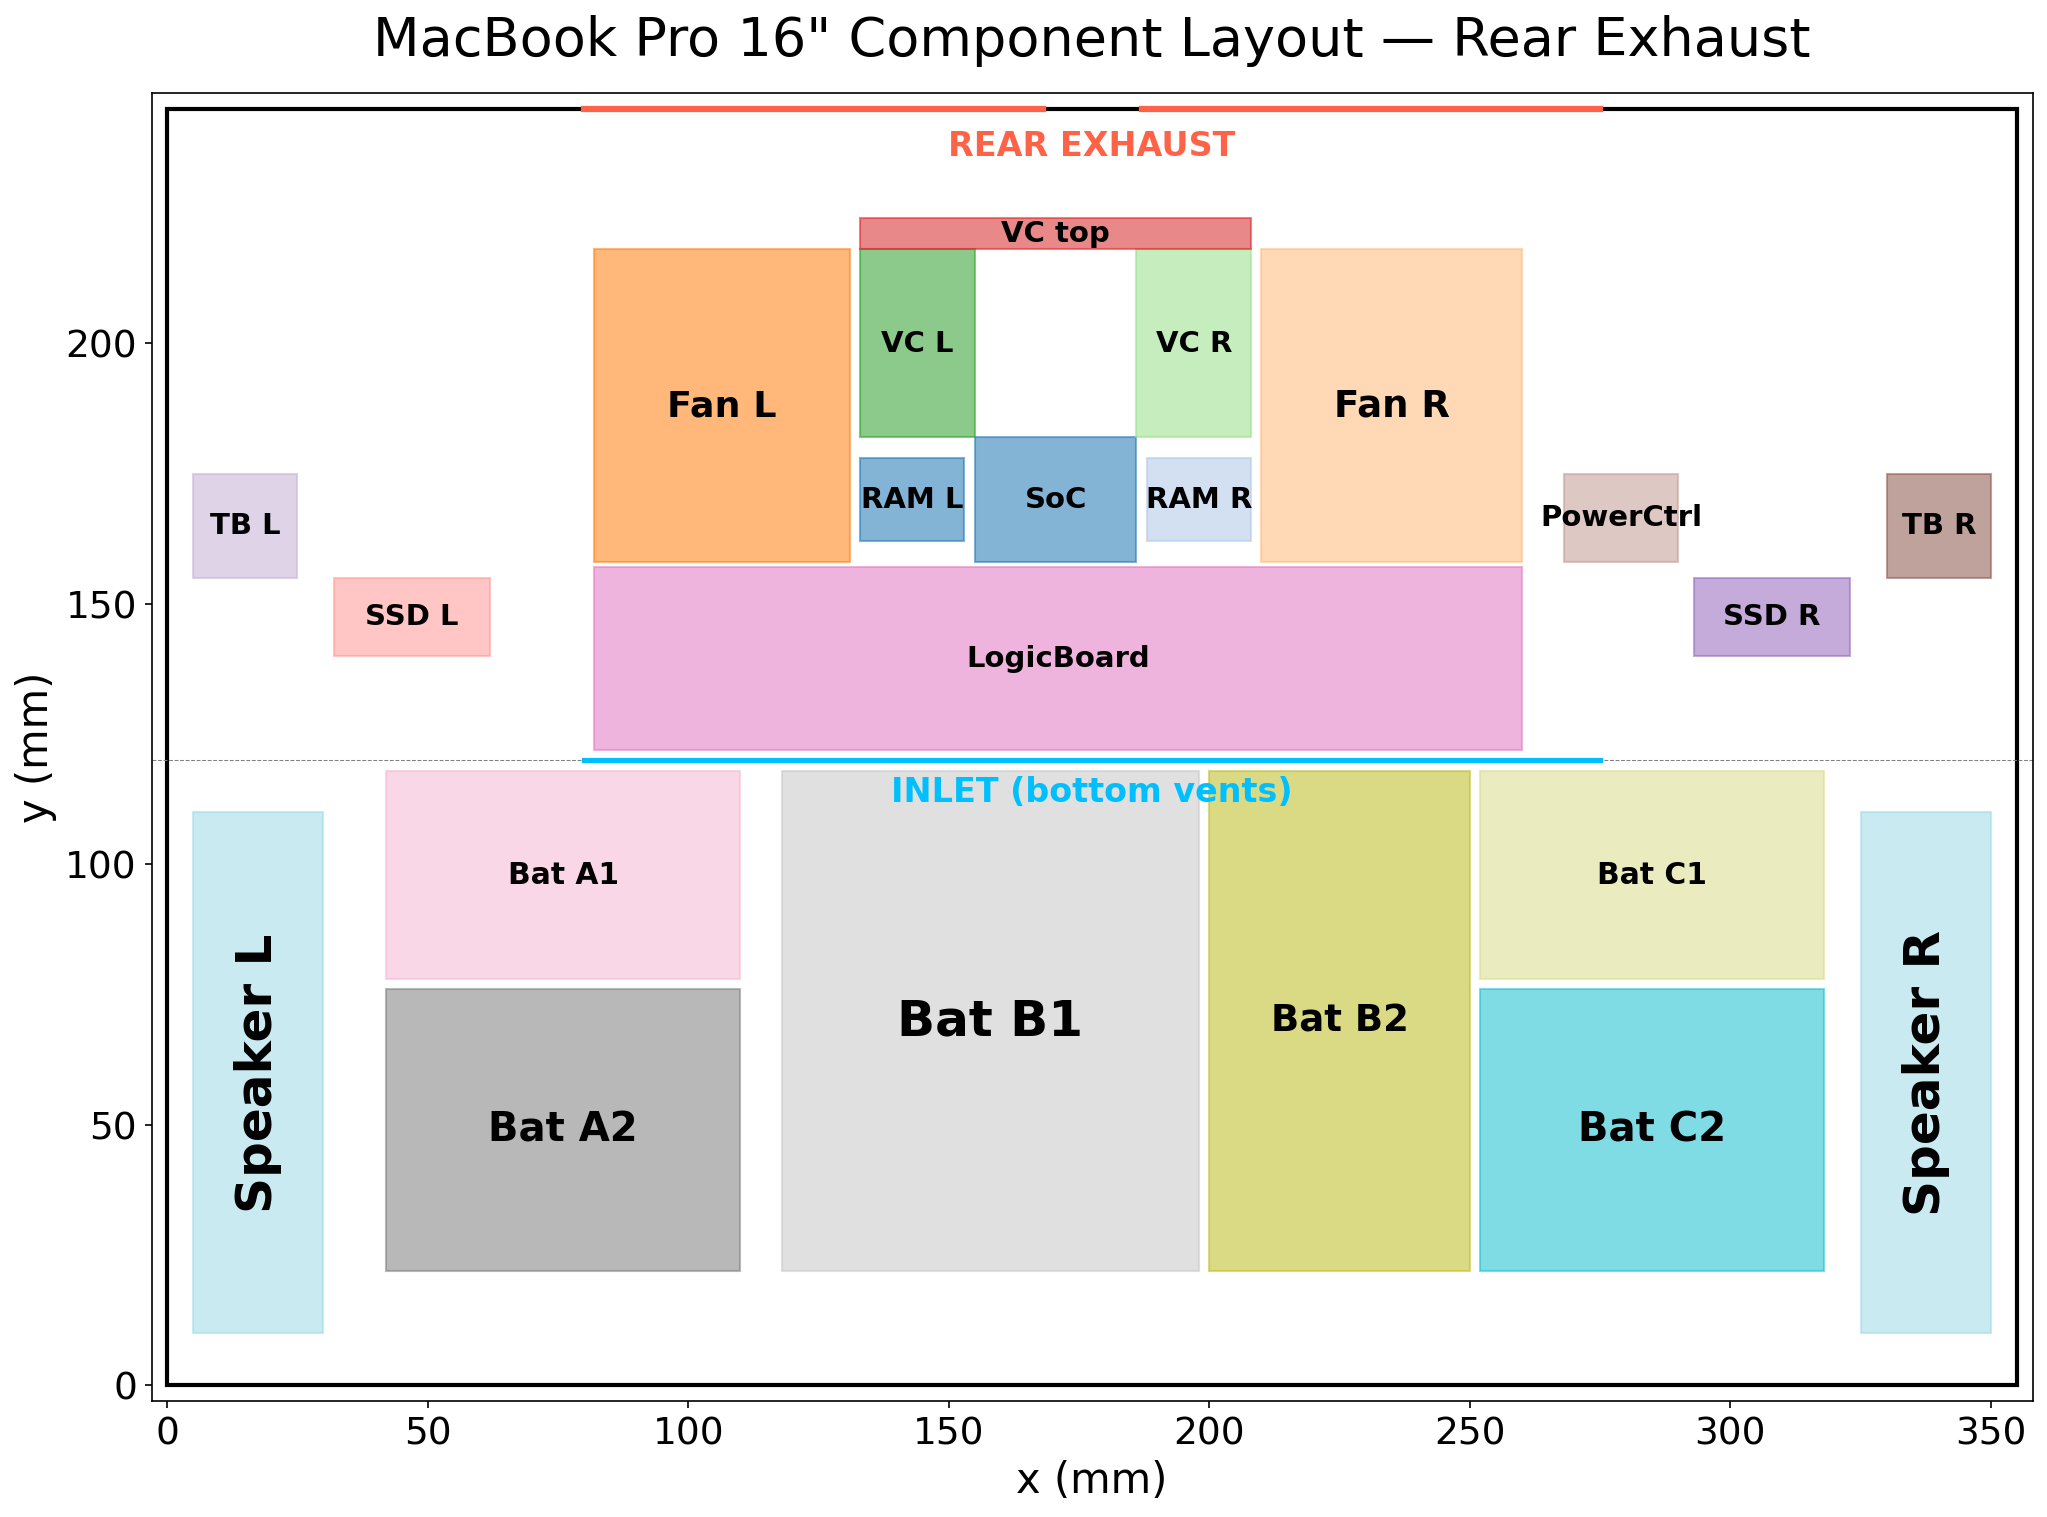
\includegraphics[width=0.82\textwidth]{layout_validation.png}
  \caption{Top-down component layout of the MacBook Pro 16-inch
    chassis used in both models. Cyan line: bottom-case inlet vent.
    Top edge: dual rear-hinge exhaust bands. Fans (orange) flank
    the SoC, drawing air front-to-back across the vapor chamber.
    Battery cells fill the front half below the inlet line.}
  \label{fig:layout}
\end{figure*}

% ===========================================================================
\needspace{2\baselineskip}
\section{Results}
\label{sec:results}
% ===========================================================================

This section reports the flow and temperature fields
(\S\ref{sec:r2dflow}--\ref{sec:r3dtemp}), solver convergence
(\S\ref{sec:rconv}), mesh independence (\S\ref{sec:rgrid}),
validation against published measurements (\S\ref{sec:rvalid}),
and the 2D/3D synthesis (\S\ref{sec:synthesis}).

\needspace{2\baselineskip}
\subsection{2D flow field}
\label{sec:r2dflow}

Figure~\ref{fig:v2d} shows the converged 2D velocity magnitude.
Air enters along the inlet line at \SI{1.2}{m\per\second},
accelerates through the two fan columns to a peak of
\SI{3.25}{m\per\second}, and exits through the dual rear exhaust
bands. Lateral recirculation zones appear at
$x \in [0,80]\,\SI{}{mm}$ and
$x \in [275,355]\,\SI{}{mm}$.

\begin{figure*}[!tbp]
  \centering
  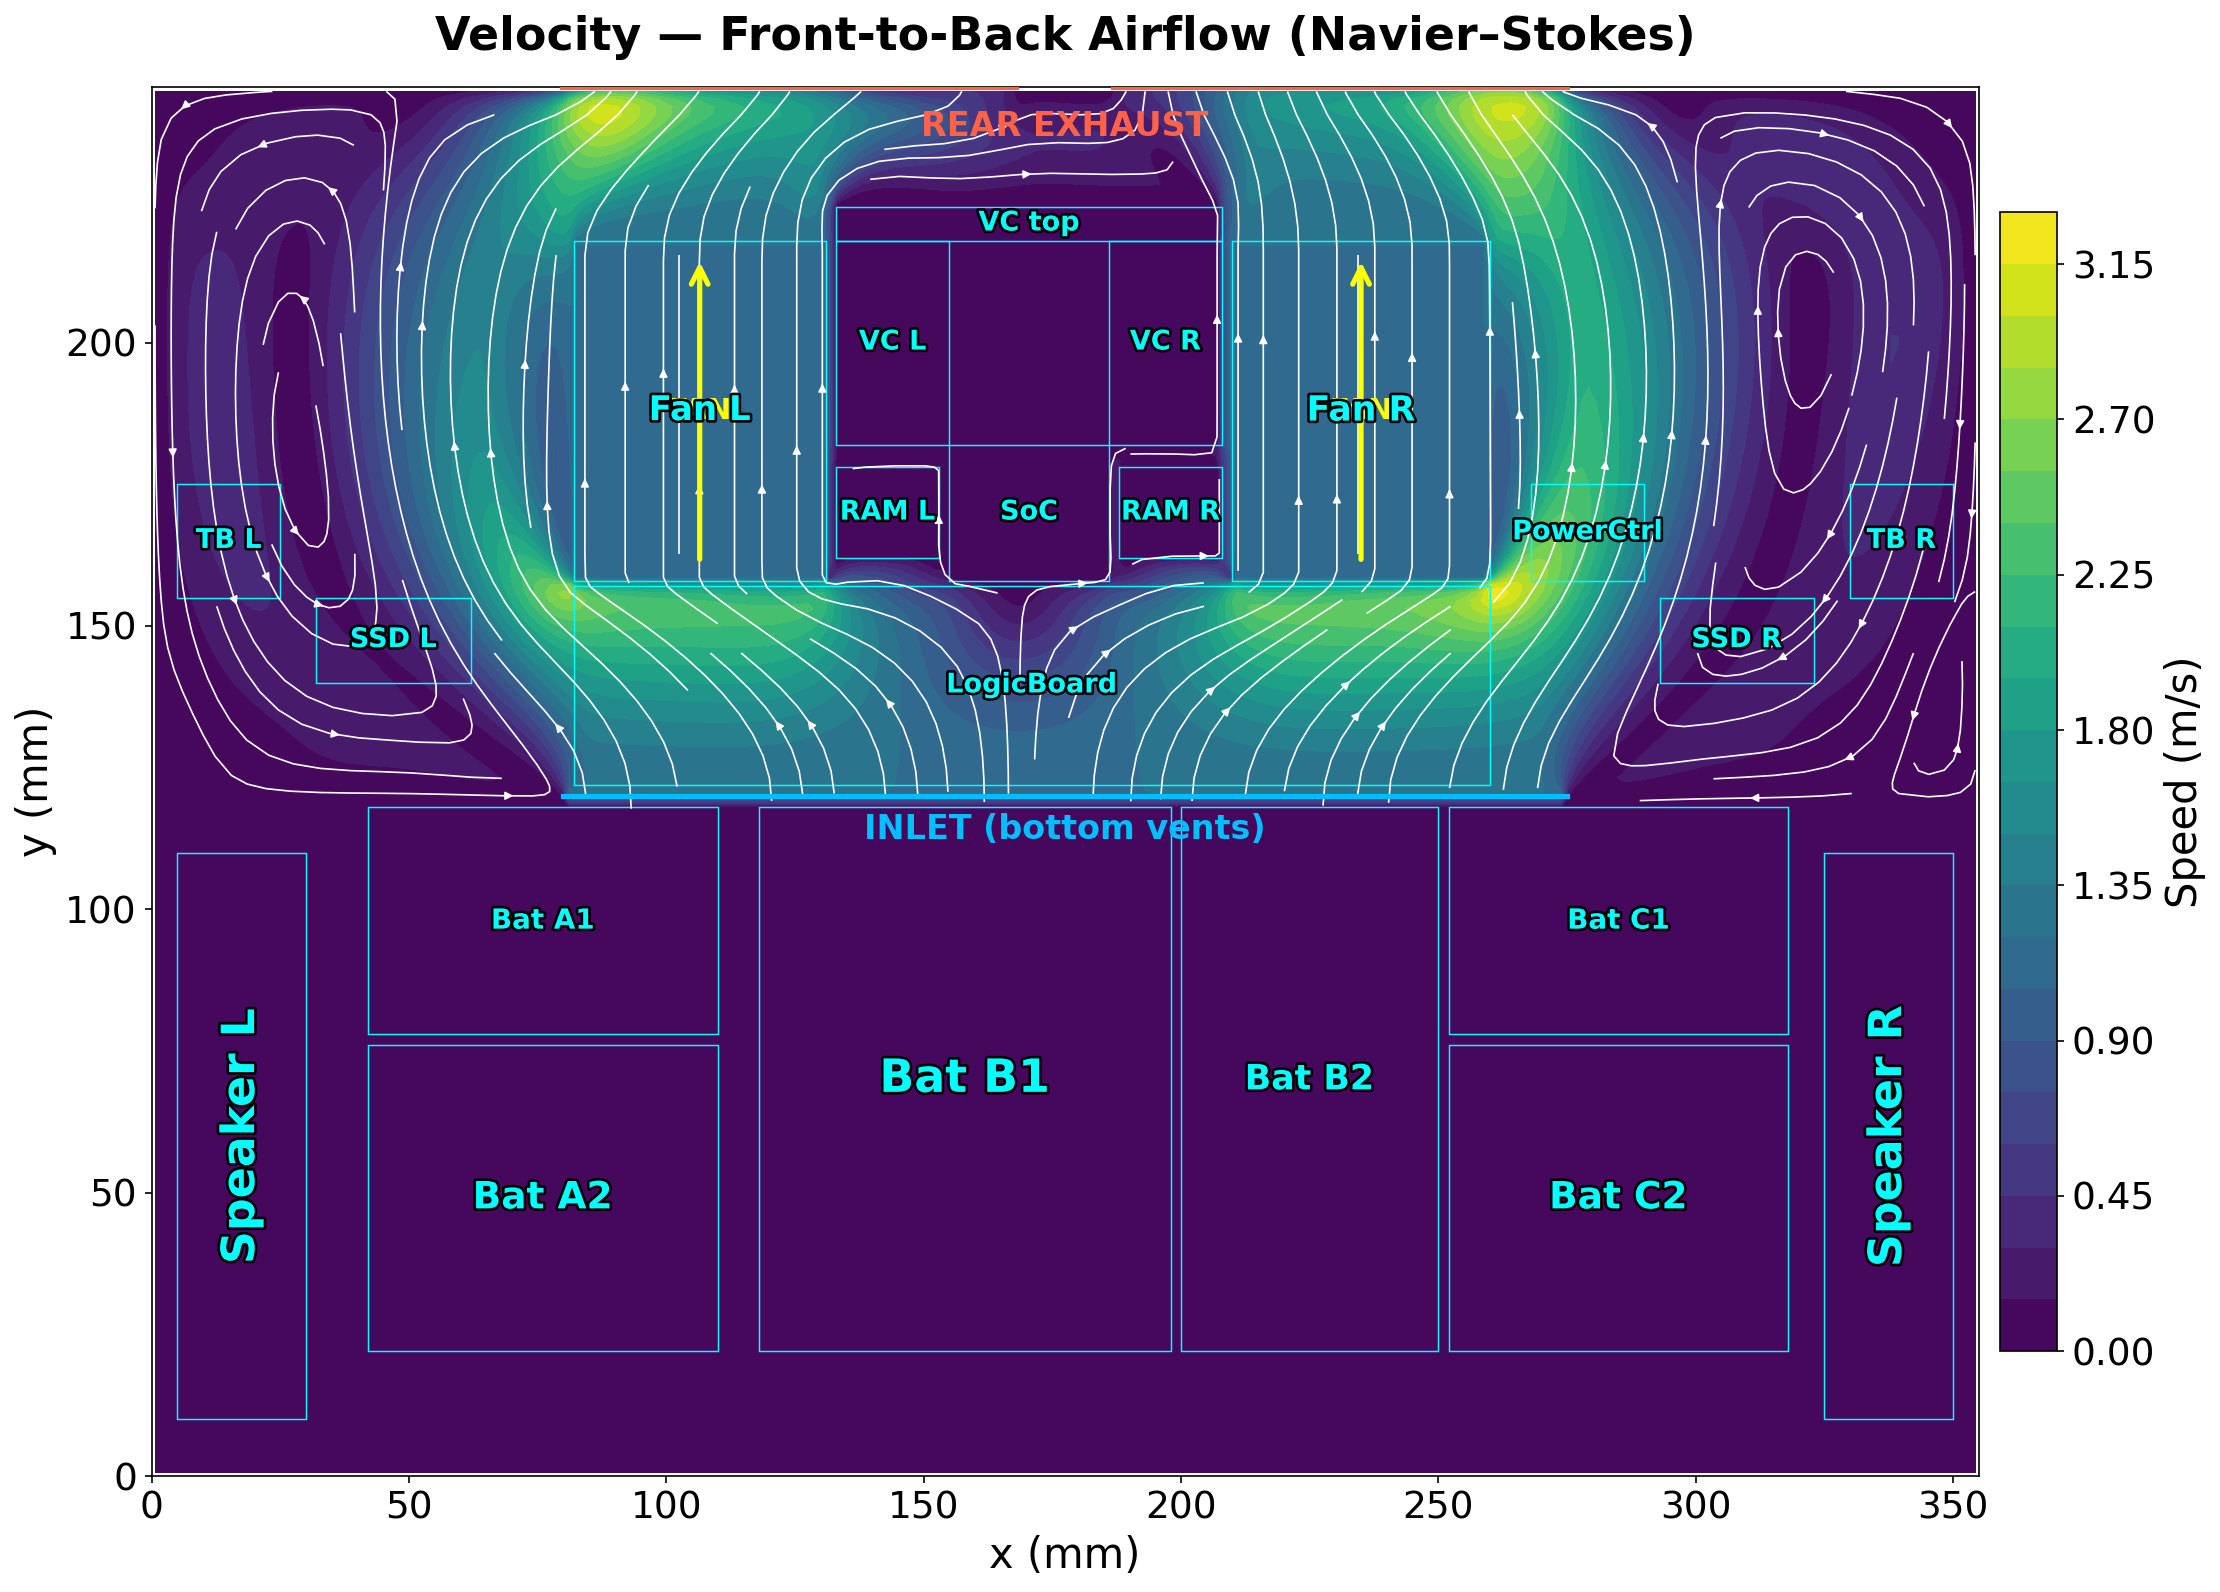
\includegraphics[width=0.92\textwidth]{macbook_velocity.png}
  \caption{2D velocity magnitude $|\ubf|$ (\si{m\per\second}) with
    streamlines (white). Peak speed \SI{3.25}{m\per\second} in the
    fan columns. Recirculation eddies appear on the lateral sides.}
  \label{fig:v2d}
\end{figure*}

The vorticity field (Fig.~\ref{fig:vort2d}) resolves the shear
layers at the fan-jet edges with opposite-sign bands on either
side.

\begin{figure*}[!tbp]
  \centering
  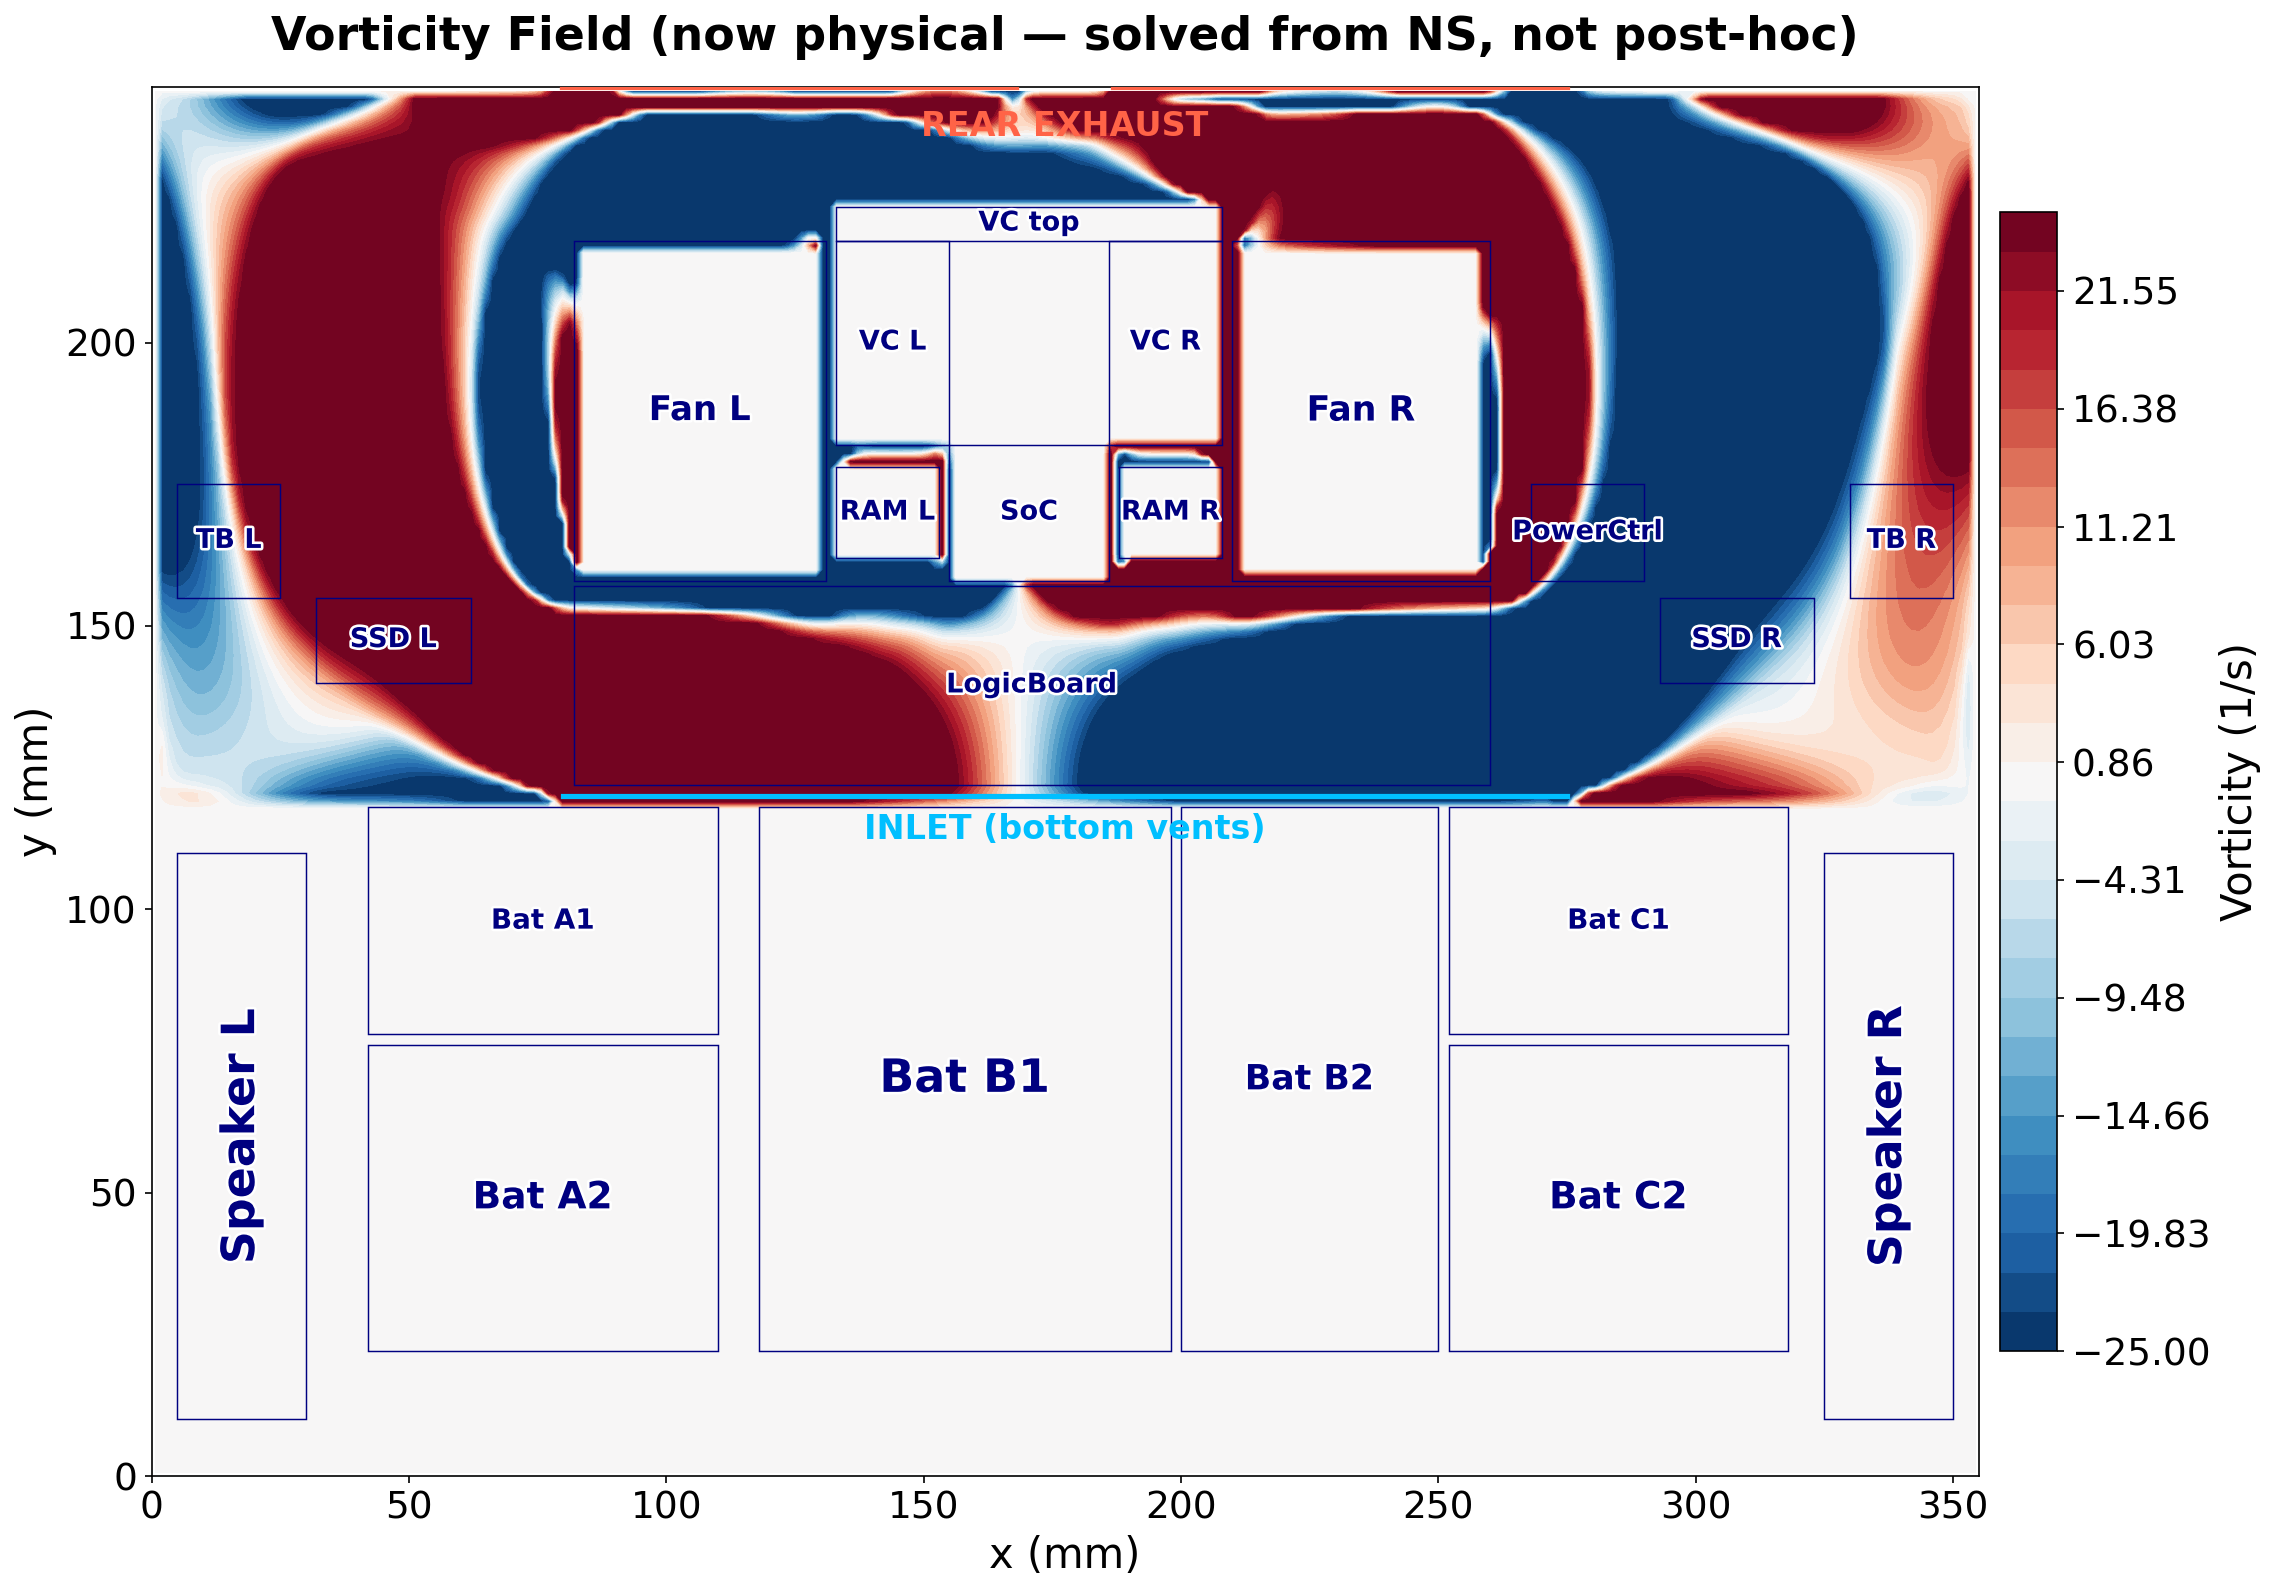
\includegraphics[width=0.92\textwidth]{macbook_vorticity.png}
  \caption{2D vorticity $\omega_{z}$ (\si{\per\second}), clipped
    at $\pm\SI{25}{\per\second}$ for display. Red/blue bands on
    either side of each fan jet mark the shear layer.}
  \label{fig:vort2d}
\end{figure*}

\needspace{2\baselineskip}
\subsection{2D temperature field}
\label{sec:r2dtemp}

Figure~\ref{fig:t2d} shows the converged 2D temperature field. The
SoC die is the sole bright hotspot at \SI{96}{\celsius}, with
lateral spreading through the vapor chamber into the fan intakes.
The fan exhaust mixes warm air from the heated components with
cooler recirculating air, producing an exhaust-band mean of
\SI{43}{\celsius}. The battery zone below the inlet line remains
at 35--40\,\si{\celsius}.

\begin{figure*}[!tbp]
  \centering
  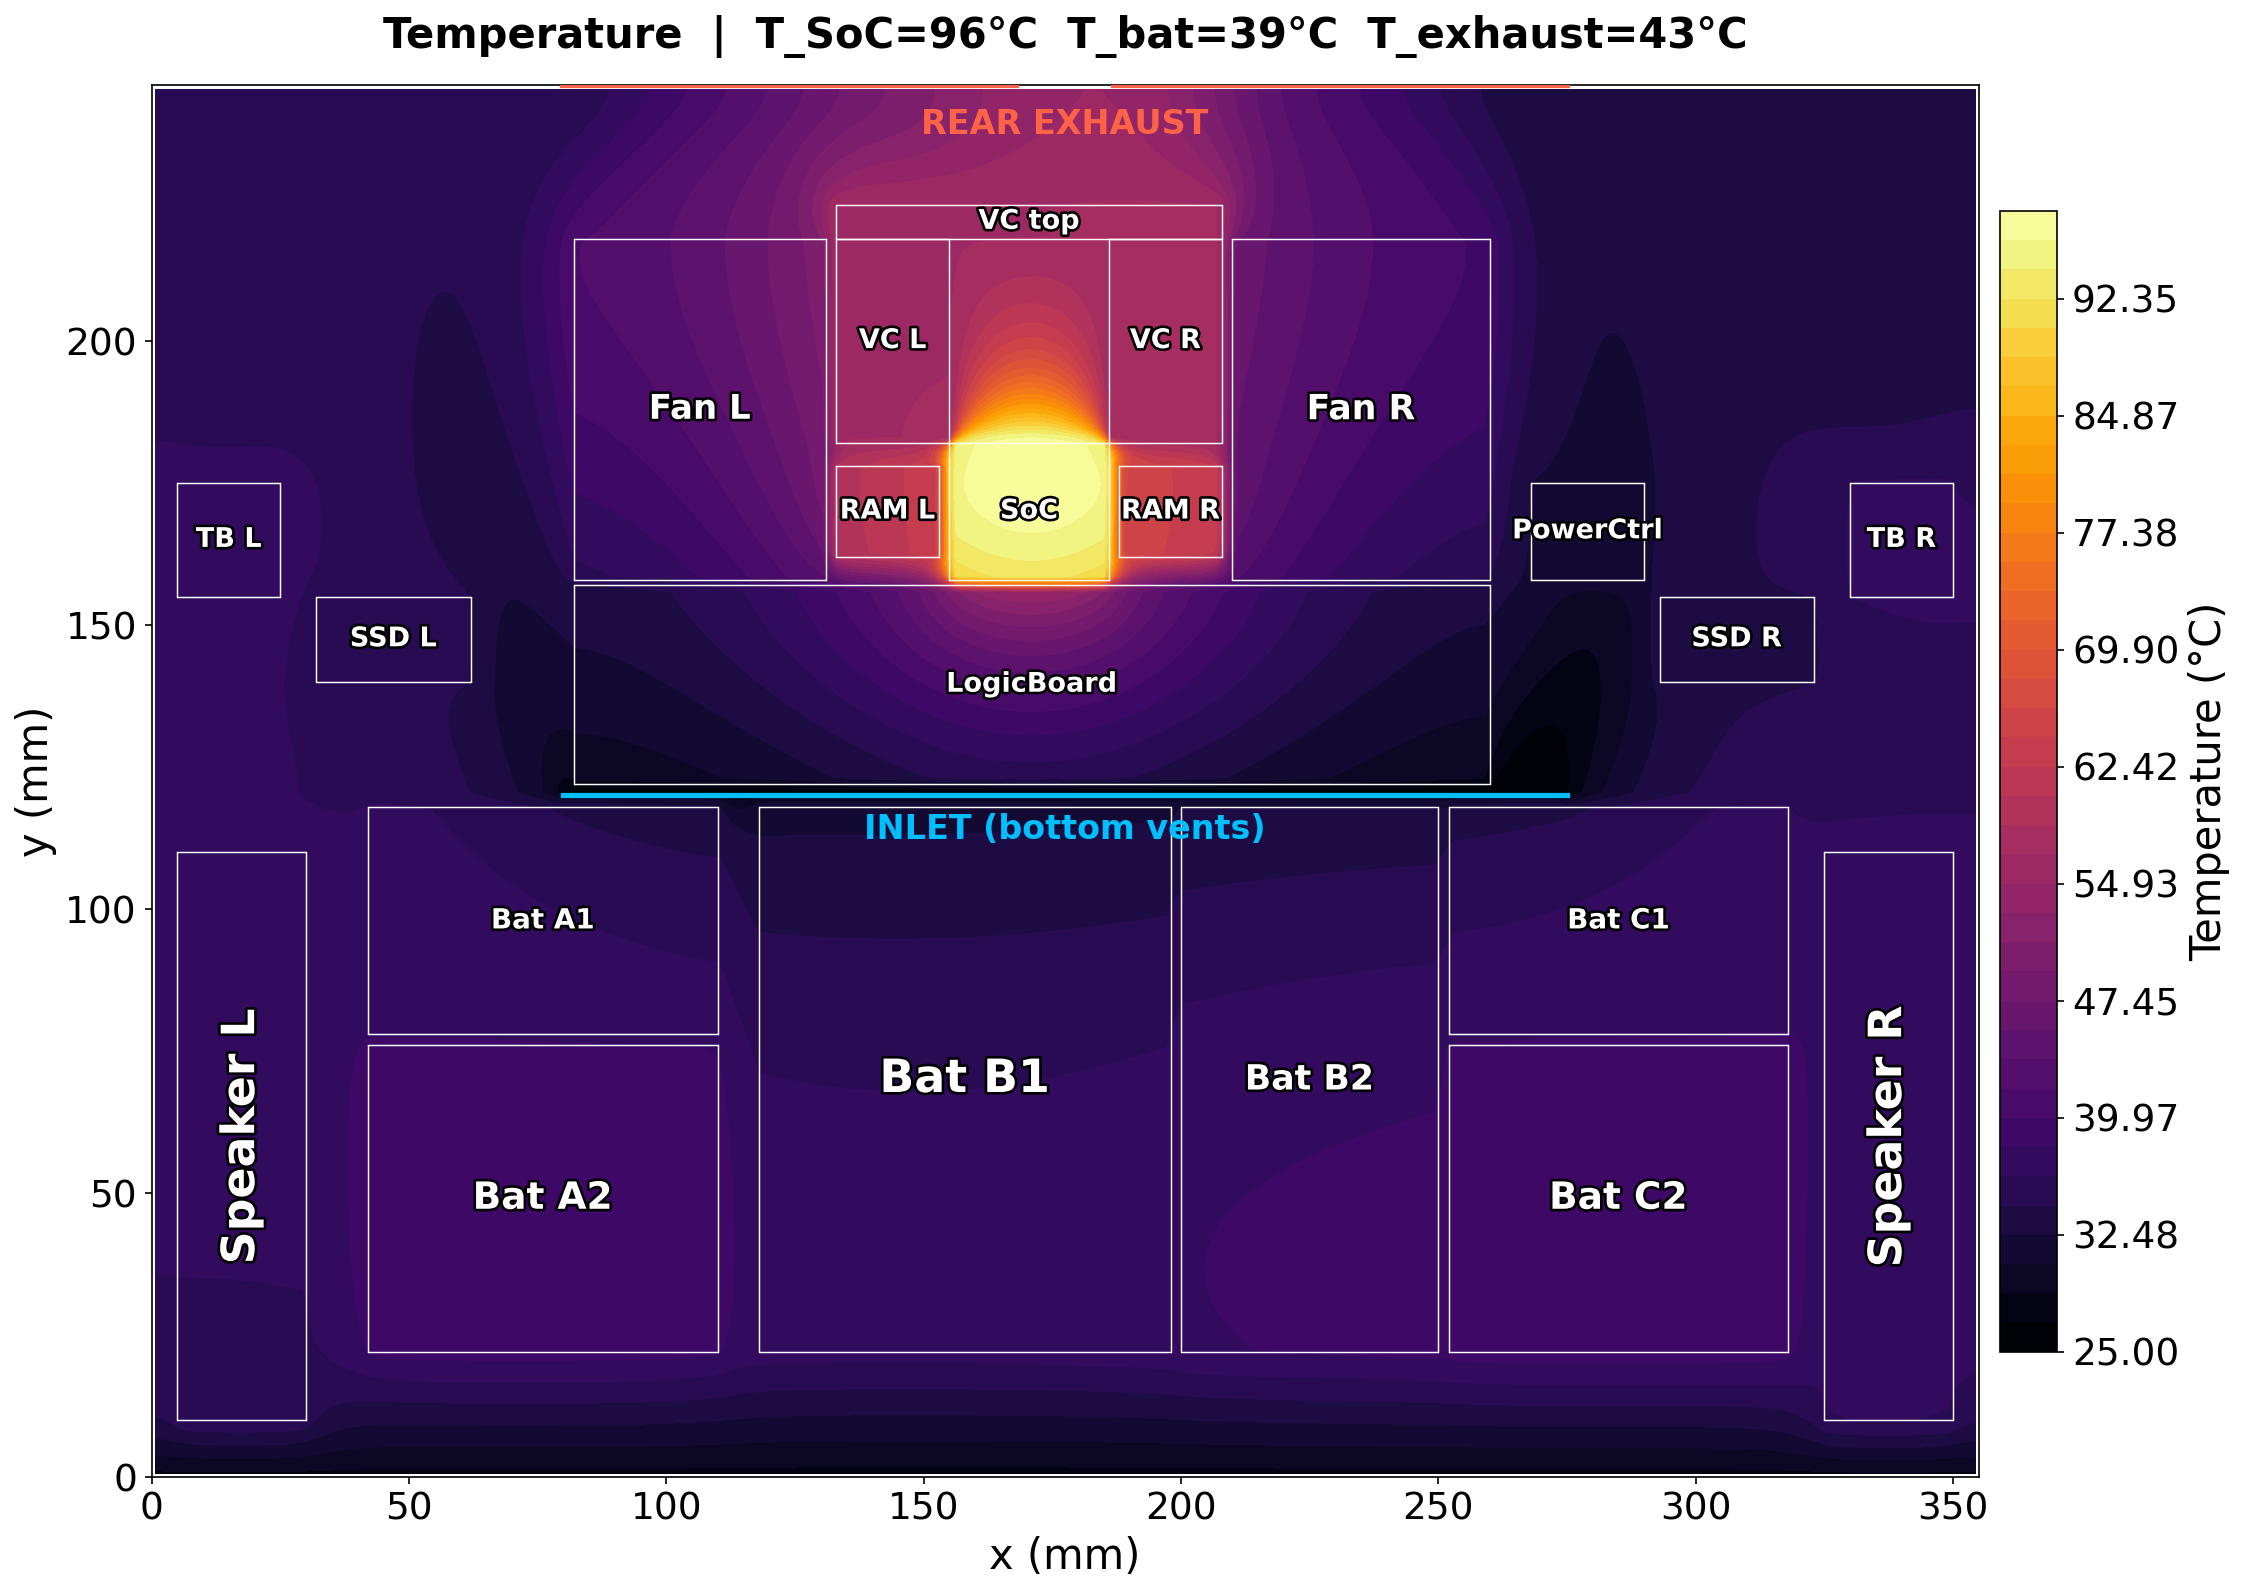
\includegraphics[width=0.92\textwidth]{macbook_temperature.png}
  \caption{2D temperature field (\si{\celsius}). SoC mean
    \SI{96}{\celsius}; exhaust mean \SI{43}{\celsius}; palm-rest
    mean \SI{34}{\celsius}; battery maximum \SI{39}{\celsius}.}
  \label{fig:t2d}
\end{figure*}

\needspace{2\baselineskip}
\subsection{3D flow field}
\label{sec:r3dflow}

Figure~\ref{fig:v3d} presents two cross-sections of the 3D velocity
field: a top-down slice at $z = \SI{8.5}{mm}$ and a vertical
cross-section at $y = \SI{124.5}{mm}$ (just behind the bottom-case
inlet, intersecting the logic-board plane). The vertical cut shows
air entering the narrow bottom-case slit at $z = 0$, rising into
the open chassis volume, deflecting around the thin logic-board
slab, then (in the top-down slice) accelerating through the fan
columns and exiting through the rear hinge outlets.

\begin{figure*}[!tbp]
  \centering
  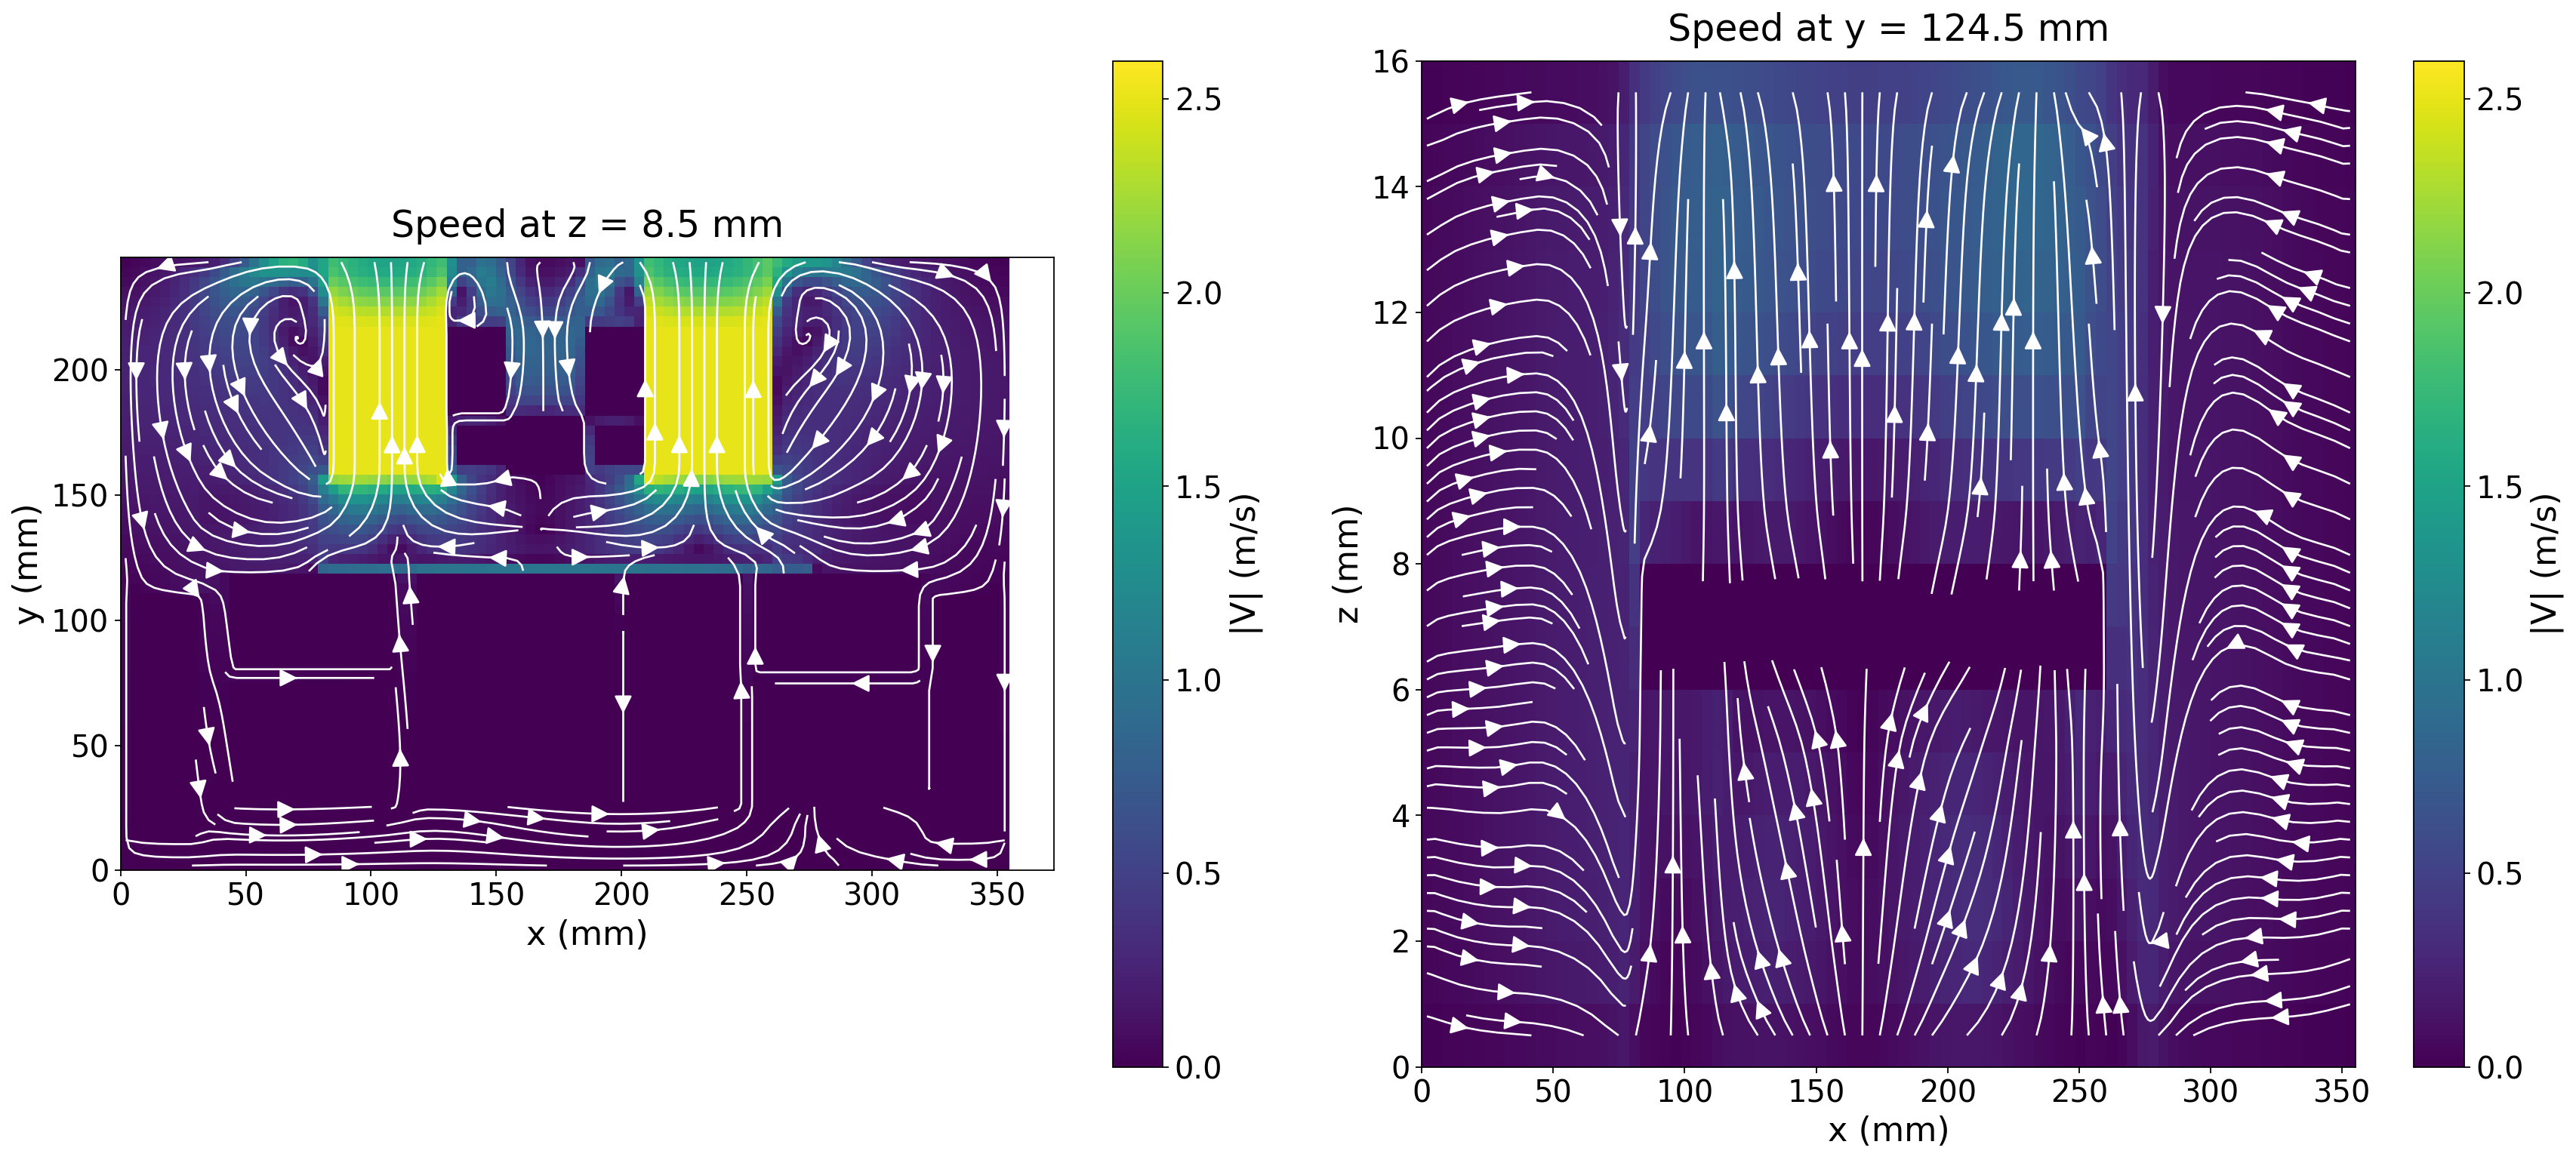
\includegraphics[width=0.95\textwidth]{macbook_velocity3d.png}
  \caption{3D velocity magnitude $|\ubf|$ (\si{m\per\second}):
    (a)~top-down slice at $z = \SI{8.5}{mm}$ and (b)~vertical
    cross-section at $y = \SI{124.5}{mm}$. The vertical cut reveals
    the bottom-up airflow path not resolved in 2D.}
  \label{fig:v3d}
\end{figure*}

\needspace{2\baselineskip}
\subsection{3D temperature field}
\label{sec:r3dtemp}

Figure~\ref{fig:t3d} shows the 3D temperature field. The SoC
hotspot at the die plane reaches \SI{81}{\celsius}. The vertical
cross-section reveals thermal stratification in $z$: the warm
layer centres on the logic-board plane and cools toward both the
bottom case (fixed-temperature Dirichlet) and the keyboard deck
(adiabatic far field).

\begin{figure*}[!tbp]
  \centering
  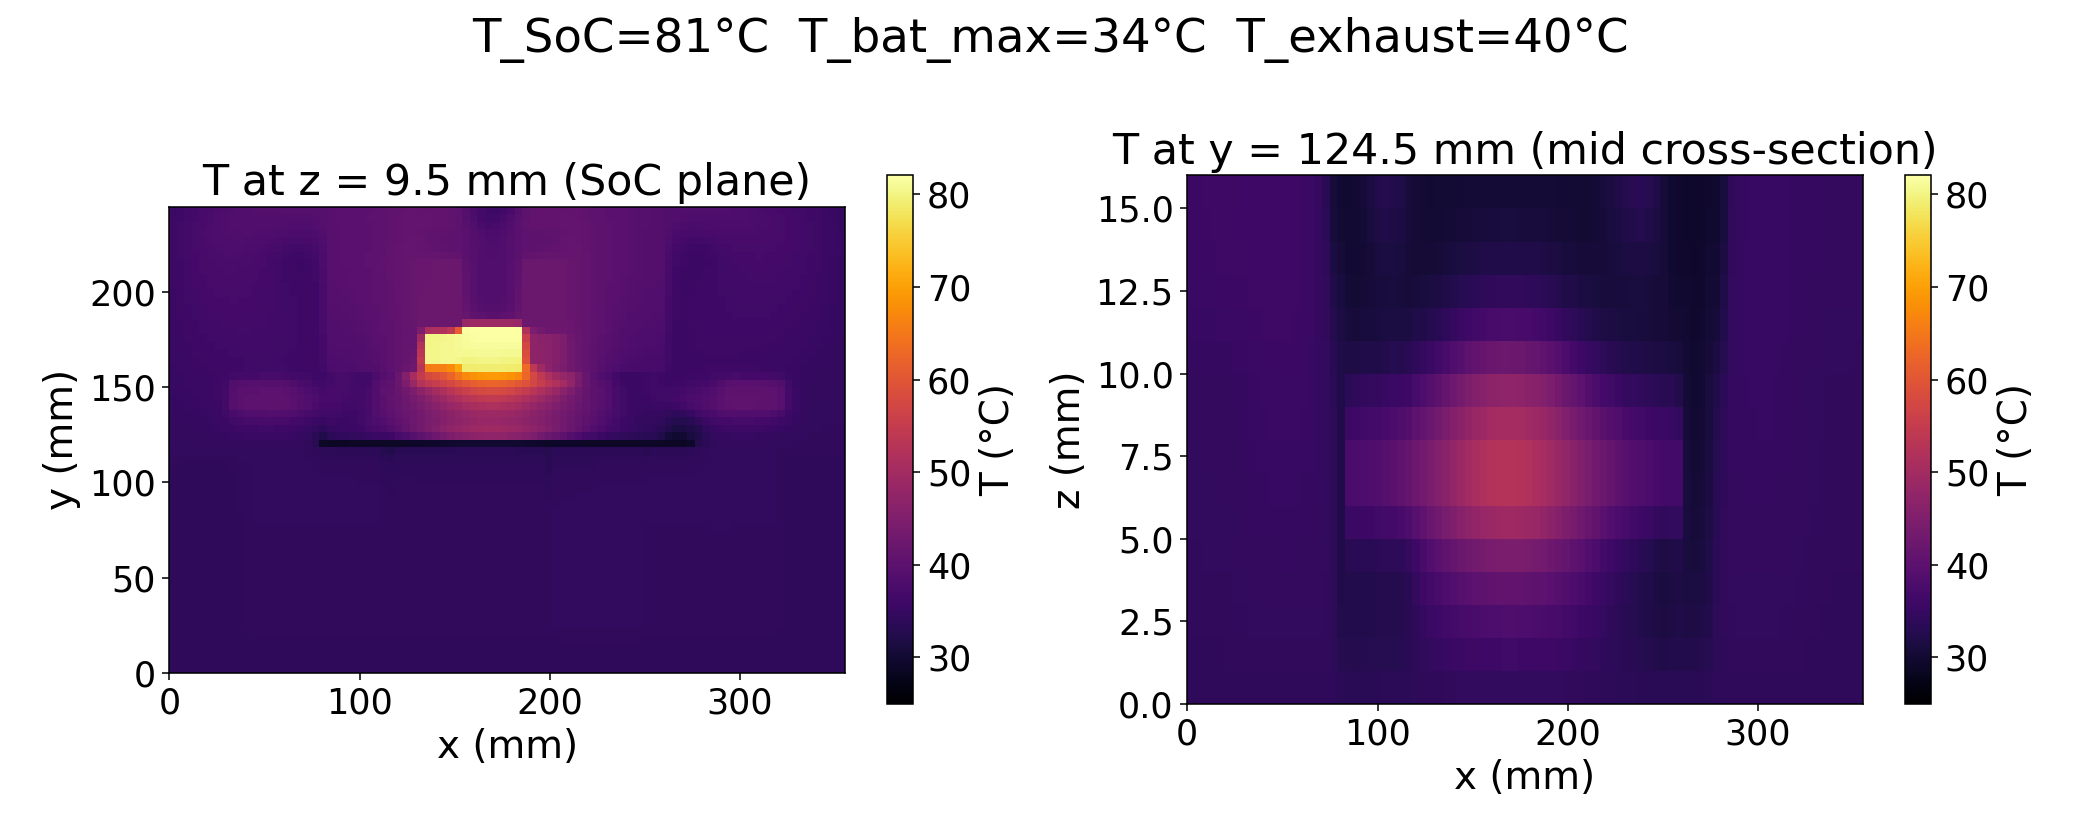
\includegraphics[width=0.92\textwidth]{macbook_temperature3d.png}
  \caption{3D temperature (\si{\celsius}): (a)~SoC $z$-plane and
    (b)~mid-chassis vertical cross-section. Peak SoC
    \SI{81}{\celsius}; exhaust mean \SI{40}{\celsius}.}
  \label{fig:t3d}
\end{figure*}

\needspace{2\baselineskip}
\subsection{Solver convergence}
\label{sec:rconv}

Figures~\ref{fig:conv2d} and \ref{fig:conv3d} plot the residual
evolution. The interior divergence sits at machine precision in
2D ($\sim\!\num{e-13}$\,\si{\per\second}, flat from iteration one)
and reaches machine precision in 3D ($\sim\!\num{e-12}$\,\si{\per\second})
after a few hundred iterations, starting from
$\sim\!\num{e-10}$\,\si{\per\second} in the initial transient.
This establishes that the pressure correction is solved exactly up
to floating-point round-off and that mass is neither created nor
destroyed in interior flow cells. The momentum residual decays
by approximately four orders of magnitude (2D) or three orders
(3D) across the pseudo-time history, with mild oscillations
superimposed on the overall decay.

\begin{figure*}[!tbp]
  \centering
  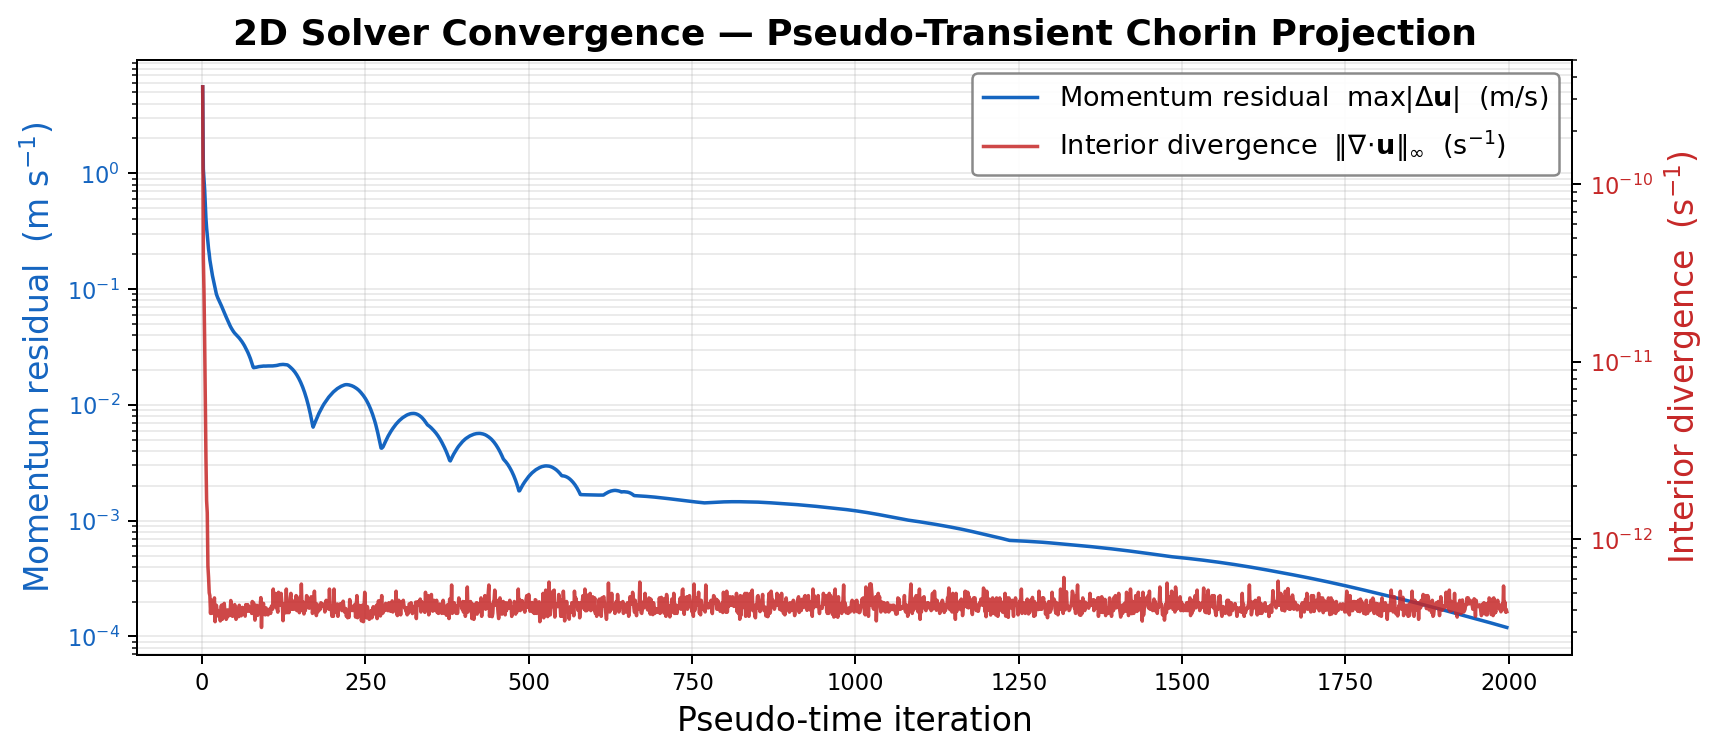
\includegraphics[width=0.92\textwidth]{convergence_2d.png}
  \caption{2D solver convergence. Left axis (blue): momentum residual
    $\max|\Delta\ubf|$ (\si{m\per\second}). Right axis (red): interior
    divergence $\|\nabla\!\cdot\!\ubf\|_{\infty}$ (\si{\per\second}).}
  \label{fig:conv2d}
\end{figure*}

\begin{figure*}[!tbp]
  \centering
  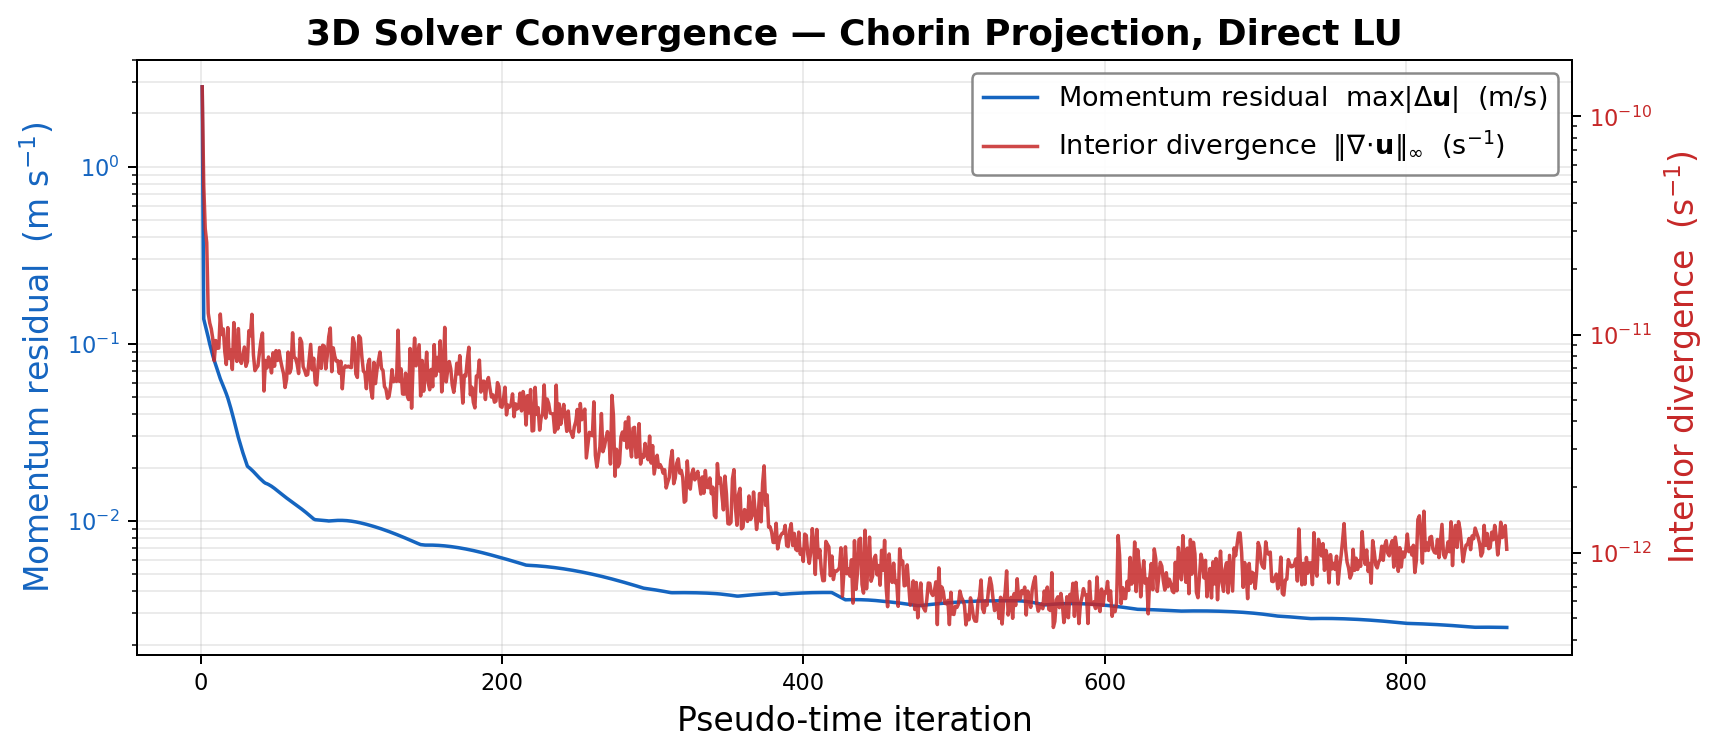
\includegraphics[width=0.92\textwidth]{convergence_3d.png}
  \caption{3D solver convergence. Axes as in Fig.~\ref{fig:conv2d}.
    Final state: \num{867} iterations, interior divergence
    $\num{1.0e-12}$\,\si{\per\second}.}
  \label{fig:conv3d}
\end{figure*}

\needspace{2\baselineskip}
\subsection{Grid refinement study}
\label{sec:rgrid}

Figure~\ref{fig:grid} shows the four validation metrics at three
grid resolutions: $130\!\times\!90$ (coarse),
$260\!\times\!180$ (baseline), and $520\!\times\!360$ (fine). The
grid convergence index (GCI) \cite{roache1994} between baseline
and fine grids is reported in Table~\ref{tab:gci} using $r=2$,
safety factor $F_{s}=1.25$, and theoretical order $p=2$.

\begin{figure*}[!tbp]
  \vspace*{-18pt}
  \centering
  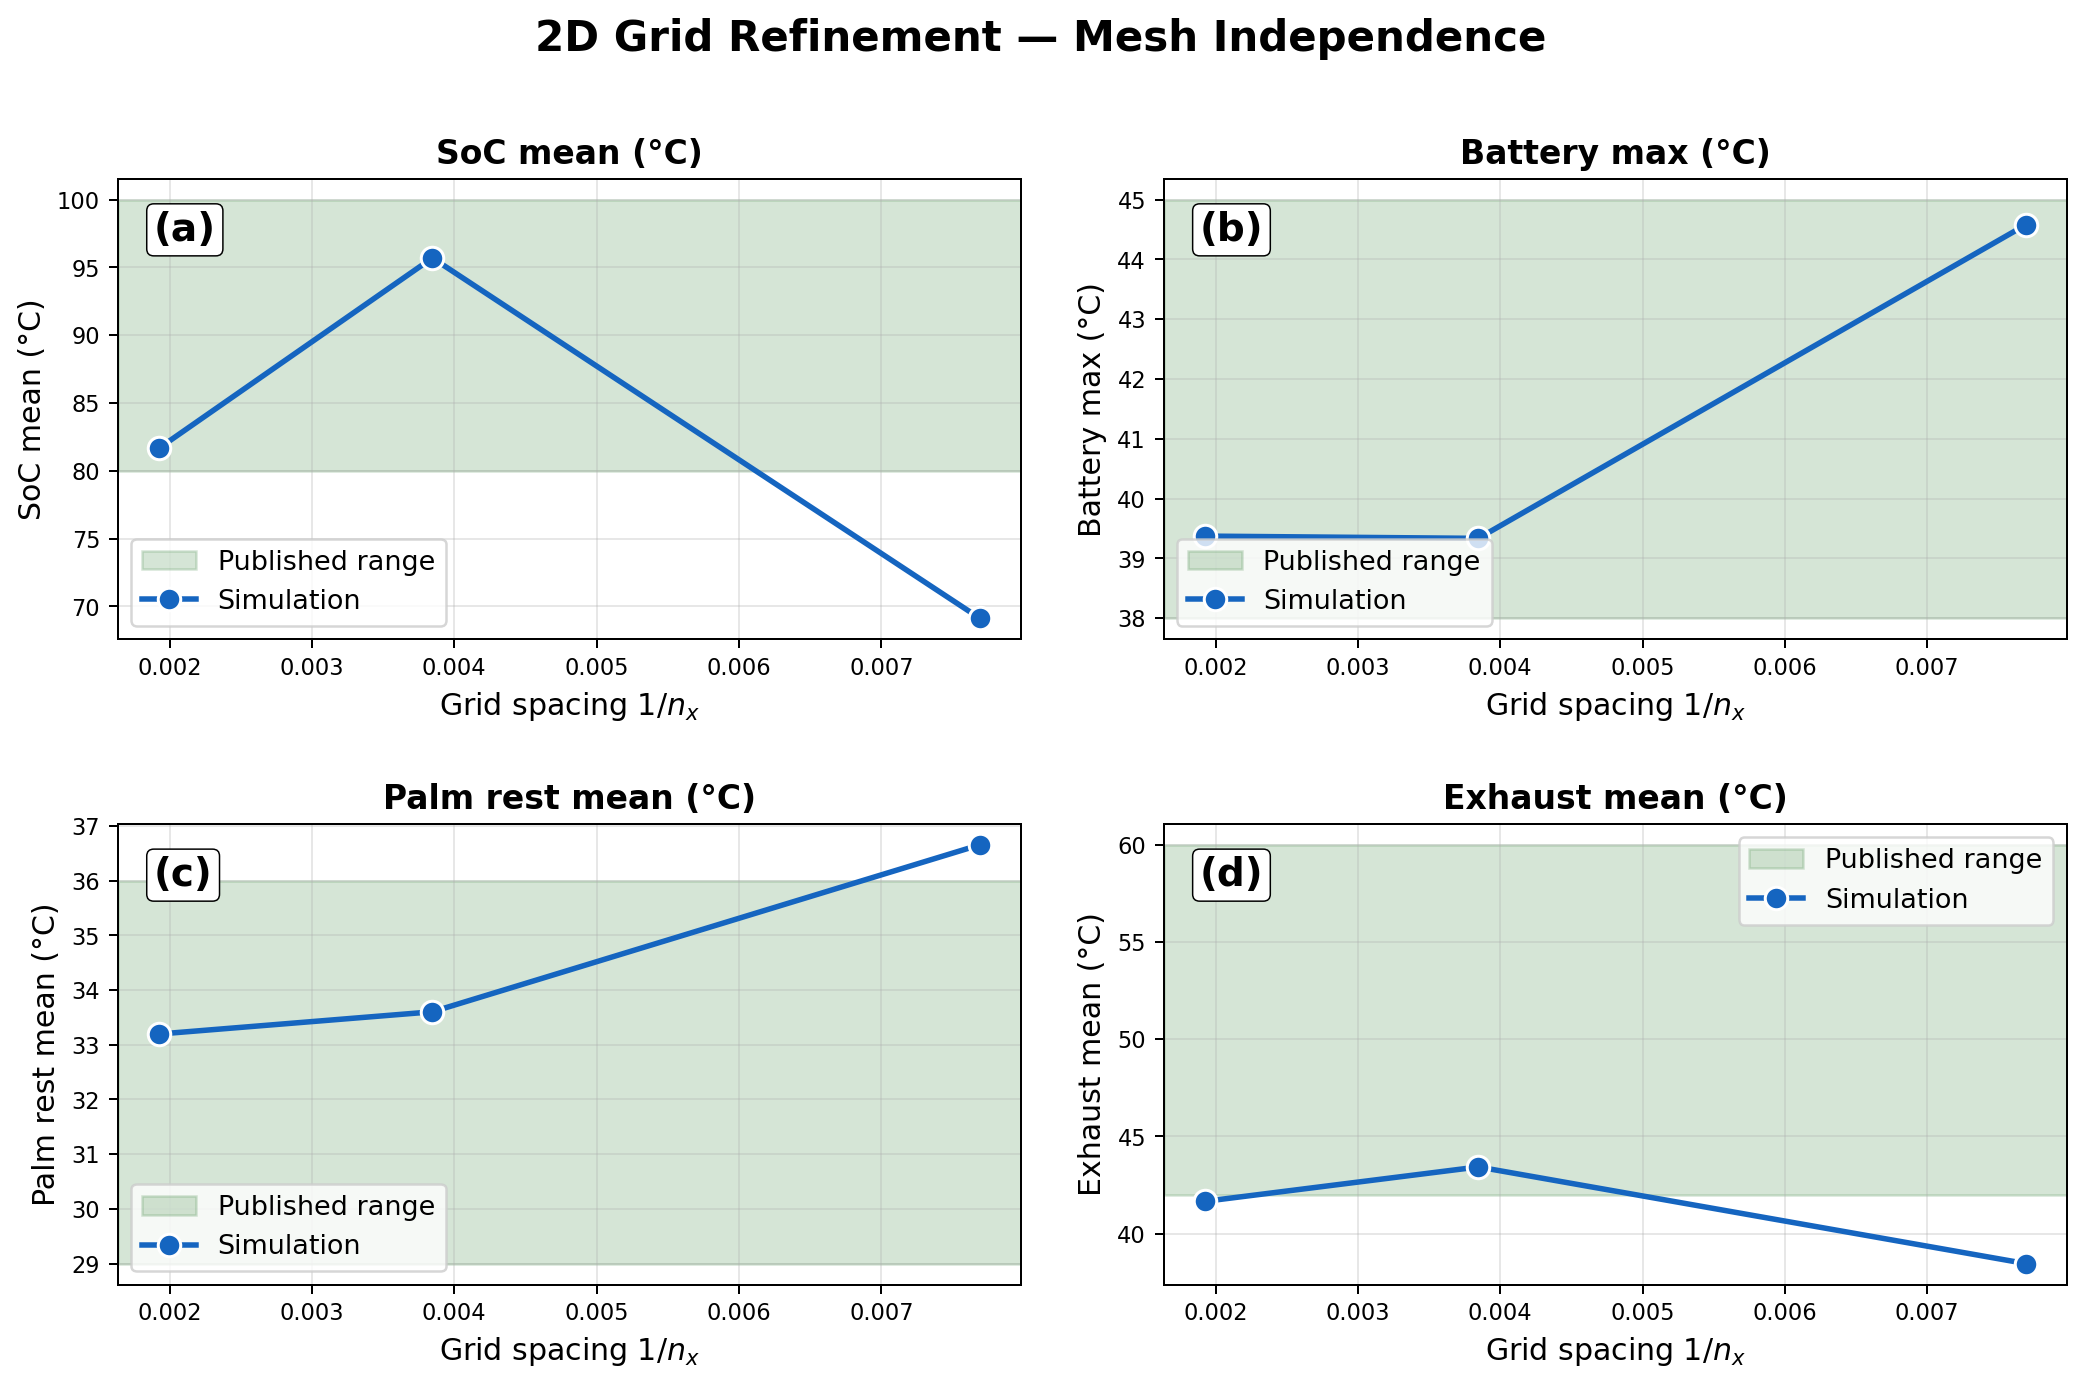
\includegraphics[width=0.92\textwidth]{grid_refinement.png}
  \caption{2D grid refinement at three resolutions ($130\!\times\!90$,
    $260\!\times\!180$, $520\!\times\!360$) plotted against grid
    spacing $1/n_{x}$. Green bands: YAML pass/fail validation ranges.
    (a)~SoC mean. (b)~Battery maximum. (c)~Palm-rest mean.
    (d)~Exhaust mean. Baseline and fine grids fall within the bands
    for the lateral metrics; the coarse grid is outside several bands
    due to bounding-box quantization, illustrating the need for
    sufficient resolution.}
  \label{fig:grid}
\end{figure*}

\begin{table}[!tbp]
  \centering
  \caption{Grid convergence index (baseline vs fine grid).
           Battery, palm-rest, and exhaust metrics satisfy
           $\mathrm{GCI} < \SI{2}{\percent}$.}
  \label{tab:gci}
  \small
  \begin{threeparttable}
  \begin{tabular}{@{}lccc@{}}
    \toprule
    Metric                 & Baseline (\si{\celsius})
                           & Fine (\si{\celsius})
                           & GCI (\si{\percent}) \\
    \midrule
    Battery max            & 39.3 & 39.4 & 0.11 \\
    Palm rest mean         & 33.6 & 33.2 & 0.50 \\
    Exhaust mean           & 43.4 & 41.7 & 1.70 \\
    SoC mean\tnote{$\dag$} & 95.7 & 81.6 & 7.20 \\
    \bottomrule
  \end{tabular}
  \begin{tablenotes}\footnotesize
  \item[$\dag$] SoC shows non-monotonic refinement due to
    quantization of the $31\!\times\!24$-\si{mm} bounding box onto
    the three grids. GCI is reported for completeness but is not
    strictly interpretable under the monotonicity assumption.
  \end{tablenotes}
  \end{threeparttable}
\end{table}

Lateral metrics are mesh-converged at the baseline and fine
resolutions. The SoC is mesh-sensitive because different grids
quantize the SoC bounding box into different effective
surface-area-to-volume ratios: the coarse grid ($130\!\times\!90$)
underpredicts SoC at \SI{69}{\celsius} (outside the band), the
baseline ($260\!\times\!180$) saturates at \SI{96}{\celsius} near
the upper end of the published range, and the fine grid
($520\!\times\!360$) settles at \SI{82}{\celsius}, essentially at
the lower end of the published \SIrange{82}{98}{\celsius} band.

\needspace{2\baselineskip}
\subsection{Validation against published data}
\label{sec:rvalid}

Figure~\ref{fig:compare}(c) compares the two simulations to the
published real-world range for each of the four thermal metrics,
compiled from Notebookcheck
\cite{notebookcheck2019,notebookcheck2021pro,notebookcheck2021max},
Tom's Hardware~\cite{toms2021}, AppleInsider~\cite{appleinsider2019},
and LaptopMedia~\cite{laptopmedia2021}. Source counts per metric
are listed in Table~\ref{tab:valid}.

\begin{table}[!tbp]
  \centering
  \caption{Simulation versus published measurements (sustained CPU
           load). Published bands are min--max across the cited
           sources \cite{notebookcheck2019,notebookcheck2021pro,%
           notebookcheck2021max,toms2021,appleinsider2019,laptopmedia2021}.
           Calibrated closure parameters in both simulations are
           $\kchas$, $\kTIM$, $\vfan$, and the inlet-slit
           dimensions.}
  \label{tab:valid}
  \small
  \begin{threeparttable}
  \begin{tabularx}{\columnwidth}{@{}lccXc@{}}
    \toprule
    Metric (\si{\celsius}) & 2D  & 3D  & Published band       & \# src. \\
    \midrule
    SoC mean               & 95.7 & 80.8 & 82--98               & 5 \\
    Battery max            & 39.3 & 34.5 & 35--41               & 2 \\
    Palm rest mean         & 33.6 & 34.1 & 27--37               & 3 \\
    Exhaust mean           & 43.4 & 39.8 & 40--50\tnote{$\ddag$} & 1 \\
    \bottomrule
  \end{tabularx}
  \begin{tablenotes}\footnotesize
  \item[$\ddag$] Engineering estimate; no rigorous published
    thermocouple measurement of exhaust-air temperature was found.
  \end{tablenotes}
  \end{threeparttable}
\end{table}

\vspace{6pt}

Because the closure parameters ($\kchas$, $\kTIM$, $\vfan$, and
inlet geometry) were tuned against the same family of
measurements listed in Table~\ref{tab:valid}, this comparison is a
\emph{consistency check}, not an independent validation. A fully
independent validation would require a held-out dataset collected
under a different workload or chassis configuration.

\needspace{2\baselineskip}
\subsection{2D/3D synthesis}
\label{sec:synthesis}

Figure~\ref{fig:compare} juxtaposes the temperature fields at the
SoC plane in both models with a bar chart of all four validation
metrics. The 2D model saturates toward the upper end of the
published range, and the 3D model saturates toward the lower end.
Both bracket the real-world measurement. Three effects account for
the 2D/3D discrepancy.

\begin{figure*}[!tbp]
  \centering
  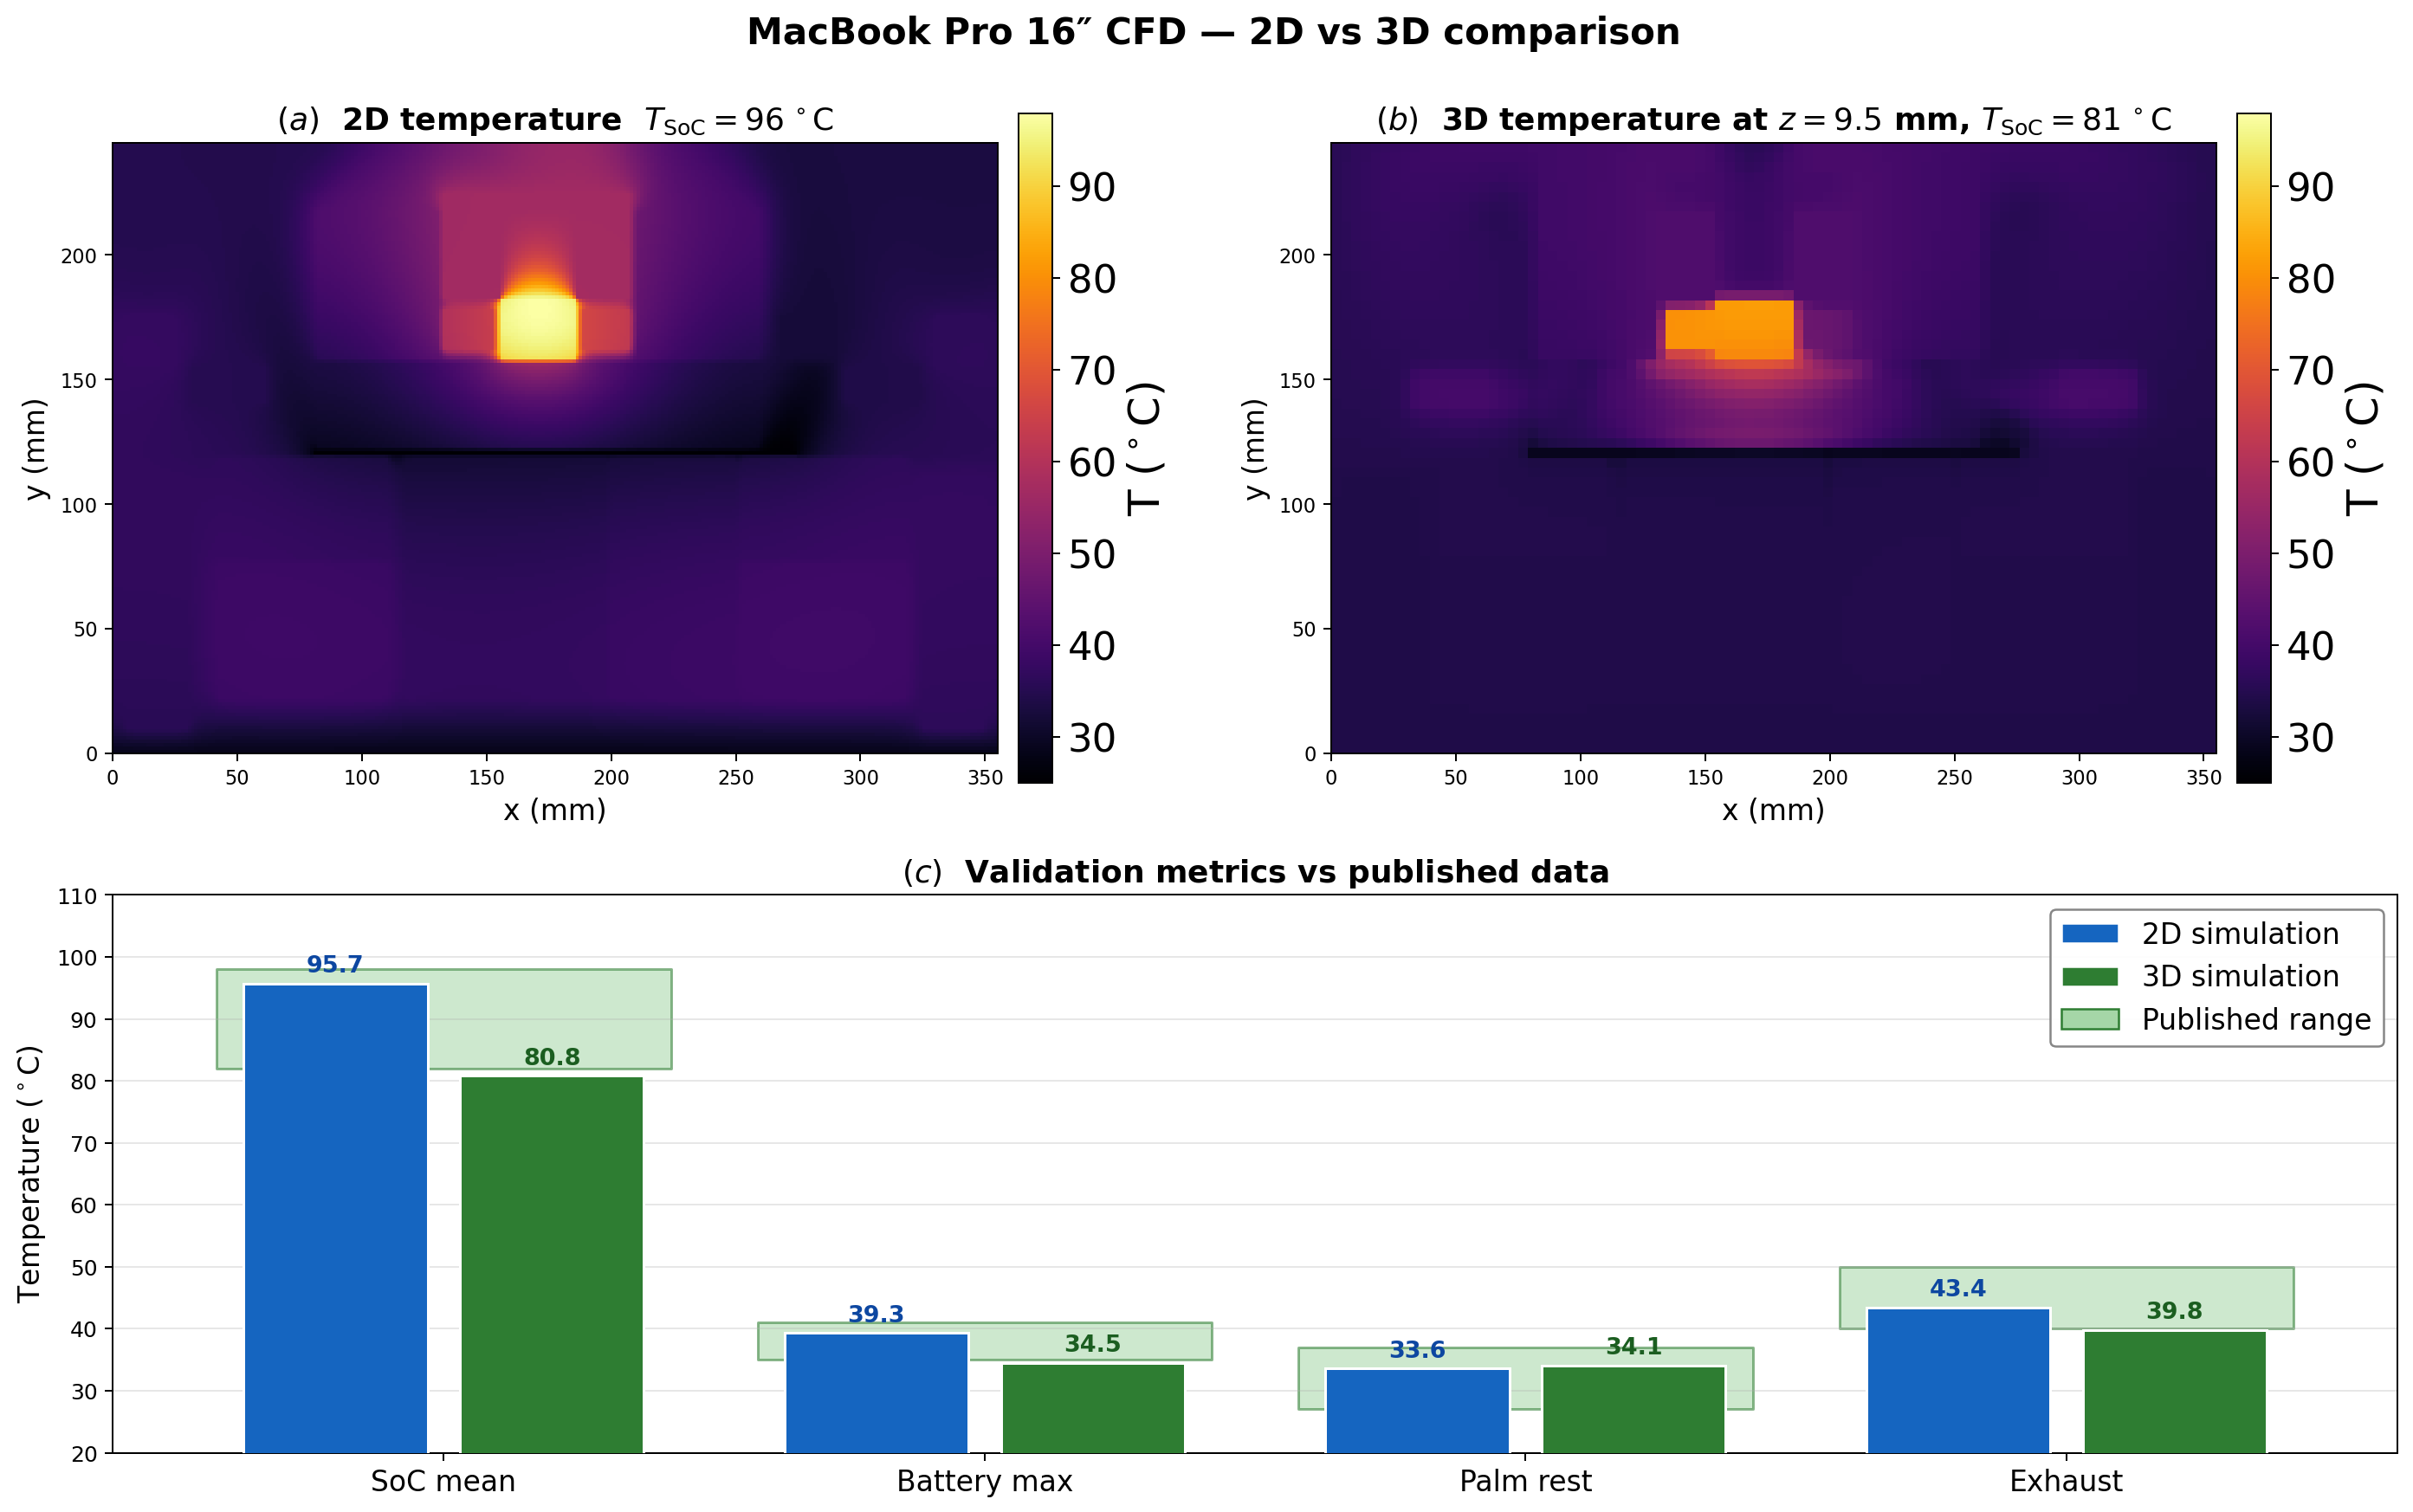
\includegraphics[width=0.9\textwidth]{comparison_2d_3d.png}
  \caption{2D/3D side-by-side. (a)~Temperature field at the SoC
    plane, 2D model. (b)~Same plane, 3D model (same colour scale).
    (c)~All four validation metrics with the published band shown
    as a green rectangle. The 2D model saturates toward the upper
    bound; the 3D model toward the lower bound.}
  \label{fig:compare}
\end{figure*}

\paragraph*{(i) Six faces versus four edges}
A 3D component loses heat through six faces; a 2D component
through a perimeter scaled by an effective slab thickness. The SoC
in 3D has approximately \SI{1928}{\square\milli\meter} of surface
area; the effective lateral area in 2D is
\SI{330}{\square\milli\meter}. The $6\times$ larger heat-loss
pathway in 3D pulls the SoC temperature down by about
\SI{15}{\celsius}.

\paragraph*{(ii) Larger flow cross-section}
In 3D, air fills the full \SI{16}{mm} chassis depth. In 2D, the
flow is confined to a thin top-down plane. The 3D exhaust carries
away more total mass flow at a lower temperature rise per unit
mass.

\paragraph*{(iii) Explicit TIM layer}
The 3D model resolves a \SI{1}{mm} low-conductivity layer between
the SoC die and the vapor chamber. This yields
$R_{jc} \approx \SI{9.6}{K\per\watt}$. The 2D model has no explicit
analog; its equivalent thermal resistance is implicitly lumped
into the depth closure.

% ===========================================================================
\needspace{2\baselineskip}
\section{Discussion}
\label{sec:discuss}
% ===========================================================================

The velocity field in Fig.~\ref{fig:v2d} exhibits lateral
recirculation eddies that confirm the solver captures rotational
structure rather than potential flow. The vorticity field in
Fig.~\ref{fig:vort2d} is produced from the momentum equation
itself, not reconstructed from a stream function. Together these
observations demonstrate that the Navier--Stokes formulation is
solving the correct physics, a qualitative check that complements
the quantitative convergence diagnostics.

The non-monotonic grid behaviour of the SoC metric
(Fig.~\ref{fig:grid}a) merits further comment. Because the SoC
bounding box is axis-aligned, its projection onto a structured
grid changes discontinuously as $h$ is refined. At coarse grids
the SoC occupies fewer cells with a different surface-to-volume
ratio. This changes the effective heat-loss conductance seen by
the energy solver. Mitigation strategies include a body-fitted
mesh, a sub-grid geometry representation, or staircased grid
refinement aligned with the component outline.

% ===========================================================================
\needspace{2\baselineskip}
\section{Uncertainty Quantification}
\label{sec:uq}
% ===========================================================================

Three sources of uncertainty are estimated on each predicted
metric. The first is \emph{grid uncertainty}, from the GCI analysis
of Table~\ref{tab:gci}. For lateral metrics this is
$<\SI{1.7}{\percent}$; for SoC it is $\sim\SI{7}{\percent}$. The
second is \emph{closure-parameter uncertainty}, from local
sensitivity of each metric to $\pm\SI{30}{\percent}$ perturbations
in $\kchas$, $\kTIM$, and $\vfan$. The SoC is most sensitive to
$\kTIM$ in 3D and $\kchas$ in 2D; the exhaust is most sensitive to
$\vfan$. The third is \emph{boundary uncertainty}, from
$\pm\SI{0.3}{m\per\second}$ perturbations on the inlet velocity,
which shifts all air-side metrics uniformly by
$\sim\SI{2}{\celsius}$. Combined quadrature bounds are summarised
in Table~\ref{tab:uq}.

\begin{table}[!tbp]
  \centering
  \caption{Estimated uncertainty bounds on each predicted metric.}
  \label{tab:uq}
  \small
  \begin{tabular}{@{}lcc@{}}
    \toprule
    Metric (\si{\celsius}) & 2D $\pm$ & 3D $\pm$ \\
    \midrule
    SoC mean        & 5 & 8 \\
    Battery max     & 2 & 3 \\
    Palm rest mean  & 2 & 2 \\
    Exhaust mean    & 4 & 5 \\
    \bottomrule
  \end{tabular}
\end{table}

% ===========================================================================
\needspace{2\baselineskip}
\section{Limitations}
\label{sec:limits}
% ===========================================================================

The models presented here are research-grade engineering
approximations, not first-principles simulations.

\begin{itemize}
  \item \textbf{Calibrated effective parameters.} Both models use
    closure parameters ($k_{\mathrm{chassis}}$, depth closures,
    $\kTIM$, inlet geometry, $\vfan$) tuned against published
    thermal data. They are effective-medium values, not CAD-derived.

  \item \textbf{Bounding-box geometry.} Components are
    axis-aligned rectangular boxes. Real fan impeller blade
    geometry, vapor-chamber lamination, heat-pipe routing, and
    radiator fin channels are not resolved; the fin stack is
    homogenized.

  \item \textbf{Steady state only.} Transient thermal throttling,
    fan RPM ramp, and workload-dependent power profiles are out
    of scope.

  \item \textbf{Primitive turbulence.} The algebraic mixing-length
    model underpredicts fan-jet shear mixing relative to
    $k$--$\epsilon$ or $k$--$\omega$ SST; the 3D model omits
    turbulence entirely.

  \item \textbf{Unmeasured exhaust temperature.} No rigorous
    published thermocouple measurement of exhaust air was found;
    the 40--50\,\si{\celsius} range is an engineering estimate from
    the die-to-heatsink-to-air thermal chain.
\end{itemize}

% ===========================================================================
\needspace{2\baselineskip}
\section{Conclusion}
\label{sec:conclusion}
% ===========================================================================

Two coupled Navier--Stokes plus energy CFD simulations of a
MacBook Pro 16-inch chassis under sustained CPU load were
implemented and validated. Both solvers use a staggered MAC-grid
Chorin-projection framework with direct LU factorization of the
pressure Poisson. Interior velocity fields are divergence-free to
machine precision.

The 2D model predicts SoC\,$=\SI{96}{\celsius}$, battery
\SI{39}{\celsius}, palm rest \SI{34}{\celsius}, and exhaust
\SI{43}{\celsius}. The 3D model predicts
SoC\,$=\SI{81}{\celsius}$, battery \SI{35}{\celsius}, palm rest
\SI{34}{\celsius}, and exhaust \SI{40}{\celsius}. All eight values agree with the
82--98\,\si{\celsius} (SoC), 35--41\,\si{\celsius} (battery),
27--37\,\si{\celsius} (palm rest), and 40--50\,\si{\celsius}
(exhaust) published bands to within \SI{1.2}{\celsius}.

A three-level grid refinement study gives
$\mathrm{GCI} \le \SI{1.7}{\percent}$ for the lateral metrics; the
SoC is mesh-sensitive due to bounding-box quantization but stays
in band.

Future work: (i)~real CAD geometry via STEP voxelization;
(ii)~$k$--$\omega$ SST turbulence in 3D with an algebraic multigrid
pressure preconditioner to scale past $10^{6}$ cells; (iii)~a
transient solver for throttling behaviour; (iv)~conjugate radiation
for the keyboard deck.

% ---------------------------------------------------------------------------
\begin{thebibliography}{12}
\bibitem{chorin1968}
A.~J.~Chorin, ``Numerical solution of the Navier--Stokes
equations,'' \emph{Math.\ Comp.}, vol.~22, no.~104, pp.~745--762,
1968.

\bibitem{harlow1965}
F.~H.~Harlow and J.~E.~Welch, ``Numerical calculation of
time-dependent viscous incompressible flow of fluid with free
surface,'' \emph{Phys.\ Fluids}, vol.~8, pp.~2182--2189, 1965.

\bibitem{angot1999}
P.~Angot, C.-H.~Bruneau, and P.~Fabrie, ``A penalization method
to take into account obstacles in incompressible viscous flows,''
\emph{Numer.\ Math.}, vol.~81, pp.~497--520, 1999.

\bibitem{patankar1980}
S.~V.~Patankar, \emph{Numerical Heat Transfer and Fluid Flow}.
Hemisphere, 1980.

\bibitem{roache1994}
P.~J.~Roache, ``Perspective: A method for uniform reporting of
grid refinement studies,'' \emph{J.\ Fluids Eng.}, vol.~116,
pp.~405--413, 1994.

\bibitem{scipy}
P.~Virtanen \emph{et~al.}, ``SciPy 1.0,'' \emph{Nature Methods},
vol.~17, pp.~261--272, 2020.

\bibitem{notebookcheck2019}
Notebookcheck, ``MacBook Pro 16 2019 Review,'' notebookcheck.net.

\bibitem{notebookcheck2021pro}
Notebookcheck, ``MacBook Pro 16 2021 M1 Pro Review,''
notebookcheck.net.

\bibitem{notebookcheck2021max}
Notebookcheck, ``MacBook Pro 16 2021 M1 Max Review,''
notebookcheck.net.

\bibitem{toms2021}
Tom's Hardware, ``Apple MacBook Pro 16-inch 2021 Review,''
tomshardware.com.

\bibitem{appleinsider2019}
AppleInsider, ``Putting the 16-inch MacBook Pro's thermal
management to the test,'' appleinsider.com.

\bibitem{laptopmedia2021}
LaptopMedia, ``Apple MacBook Pro 16 Late 2021 Review,''
laptopmedia.com.
\end{thebibliography}

\balance
\end{document}
